\cotefile{67}
\scanpage{2}
Chirurgie des \unsure{surfaces}
conformes \unsure{I} \unsure{---}

197\unsure{8|6} ou 77 ?)
% archive foliation: 1
\scanpage{3}
Chirurgie des surfaces conformes.

1) \uline{Découpage} : \unsure{Découpe} d'une surface conforme \deleted{\unsure{sans bord}} (\unsure{évt}
avec bord) suivant un sous-1-complexe rectifiable
compact : On trouve une surface conforme à \deleted{\unsure{un}}
bord, avec morceau \inserted{\deleted{compact}} de bord compact marqué

2) \uline{Recollage} : À partir d'une surface conforme
(avec bord \deleted{\unsure{si on veut}}) et d'un morceau
compact du bord, et une relation d'équivalence
``admissible'' \inserted{(au sens rectifiable)} sur le bord, \deleted{\unsure{on a}} on trouve
une surface conforme avec bord\ldots

3) \uline{\unsure{Rétrécissage}}
\[
\underset{\substack{1\text{-compl.}\\\text{cpt}}}{K}
\subset
\underset{\text{s. conforme avec bord}\ \unsure{?}}{X}
\]
$\widetilde X$ découpé de $X$ suivant $K$, $\partial'\widetilde X$ partie distinguée
du bord, on choisit un \inserted{multi-}anneau autour de
$\partial'\widetilde X$, \deleted{\unsure{soit alors}} (un germe
de \unsure{tel anneau} autour
d'une composante
$(\partial'_{\unsure{i}}\widetilde X)_{\unsure{i}}$ \unsure{revient} : la donnée
d'une structure Riemannienne
\deleted{régulière} \inserted{rectifiable} de long. totale $1$
sur celle-ci\ldots)

\figure{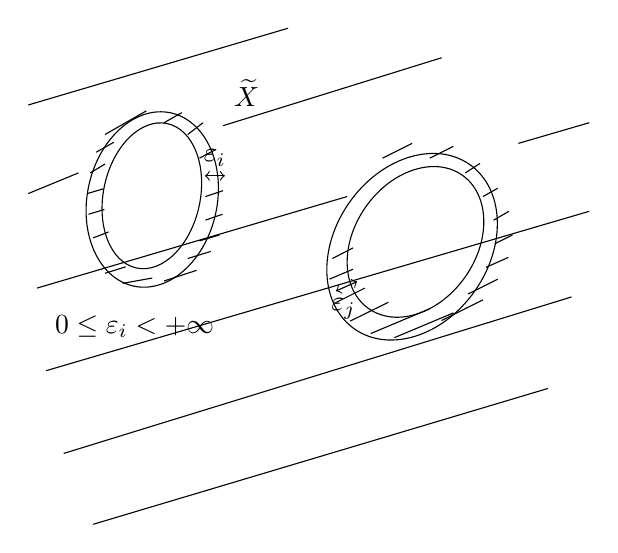
\begin{tikzpicture}[x=0.75cm,y=0.75cm]
\draw (-.3,2.8)--(4.1,4.1);
\draw (-.3,1.3)--(.55,1.65) (3.0,2.45)--(6.7,3.6);
\draw (-.15,-.3)--(5.1,1.25) (8.0,2.15)--(9.2,2.5);
\draw (0,-1.7)--(9.2,1.0);
\draw (.3,-3.1)--(8.9,-.45);
\draw (.8,-4.3)--(8.5,-2.0);
\draw[rotate around={-12:(1.8,1.2)}] (1.8,1.2) ellipse (1.1 and 1.5);
\draw[rotate around={-12:(1.8,1.2)}] (1.78,1.26) ellipse (.82 and 1.25);
\draw (1.0,2.3)--(1.7,2.7) (.85,2.0)--(1.15,2.17) (.75,1.65)--(1,1.8)
(.7,1.3)--(.97,1.38) (.72,.95)--(.99,1.03) (.8,.55)--(1.06,.65)
(1,-.05)--(1.35,.06) (1.3,-.22)--(1.8,-.13) (2,-.18)--(2.55,0)
(2.4,.2)--(2.79,.32) (2.6,.5)--(2.94,.6) (2.7,.85)--(2.99,.95)
(2.7,1.25)--(3,1.35) (2.6,1.9)--(2.88,2.05) (2.4,2.3)--(2.66,2.5)
(2.0,2.5)--(2.3,2.67);
\draw[rotate around={-35:(6.2,.4)}] (6.2,.4) ellipse (1.3 and 1.7);
\draw[rotate around={-35:(6.2,.4)}] (6.2,.5) ellipse (1.03 and 1.38);
\draw (4.85,.2)--(5.2,.38) (4.8,-.15)--(5.2,.02) (4.9,-.55)--(5.4,-.3)
(5.15,-.86)--(5.8,-.54) (5.5,-1.07)--(6.5,-.65) (5.9,-1.14)--(6.9,-.72)
(6.7,-.85)--(7.4,-.5) (7.15,-.4)--(7.65,-.15) (7.45,.05)--(7.83,.22)
(7.6,.45)--(7.9,.6) (7.58,.85)--(7.84,1.0) (7.4,1.25)--(7.65,1.39)
(7.1,1.65)--(7.35,1.81) (6.5,1.9)--(6.9,2.1) (5.7,1.9)--(6.2,2.15);
\node at (3.4,3.0) {$\widetilde X$};
\draw[<->] (2.69,1.6)--(3.03,1.6);
\node[above] at (2.86,1.6) {$\varepsilon_{\unsure{i}}$};
\draw[<->] (4.91,-.35)--(5.27,-.19);
\node[below] at (5.04,-.32) {$\varepsilon_{\unsure{j}}$};
\node at (1.5,-.95) {$0\leq\varepsilon_i<+\infty$};
\end{tikzpicture}}

$\widetilde X^*$ la surface \inserted{\deleted{à bord \unsure{droit}}\inserted{\unsure{droit}}\deleted{\unsure{rectif.}}} rétrécie
\unsure{déduit} de la couronne
choisissons un isomorphisme rectifiable
$\partial'\widetilde X^*\xrightarrow{\sim}\partial'\widetilde X$ compatible avec les comp. connexes,
et utilisons la relation d'équivalence \inserted{de recollage} sur
$\partial'\widetilde X$ pour en déduire une sur $\widetilde X^*$. On
en \unsure{conclut} \deleted{$\unsure{K\subset}$} $X^*$ et $K\subset X^*$
% archive foliation: 2
\scanpage{4}
4) \uline{\unsure{Élargissage}} Opération inverse -- au lieu de
retrancher une couronne, on en rajoute une\ldots

5) Opération mixte : \uline{panachage}

On considère un voisinage tubulaire \unsure{standart|standard}
de $\partial'\widetilde X$, et dans \inserted{chaque composante $T_i$ de} celui-ci, un
cercle $\Gamma_i$, et un isom. rect.
$\Gamma_i\simeq(\partial'\widetilde X)_i$. On \deleted{\unsure{se donne}} \inserted{\deleted{définit}}
\deleted{considère}\inserted{considère} $\deleted{\unsure{\partial}}\widetilde X^{\unsure{*|\circ}}$ déduit de
$\widetilde X$ en enlevant \inserted{$\unsure{K_i}$} ``la \deleted{\unsure{intérieur}}
\deleted{de $\Gamma_i$} partie de $T_i$ entourée
par $\Gamma_i$''. On termine comme dans
3°), 4°) pour trouver $\widetilde X^*$ et $K\subset X^*$.

\figure{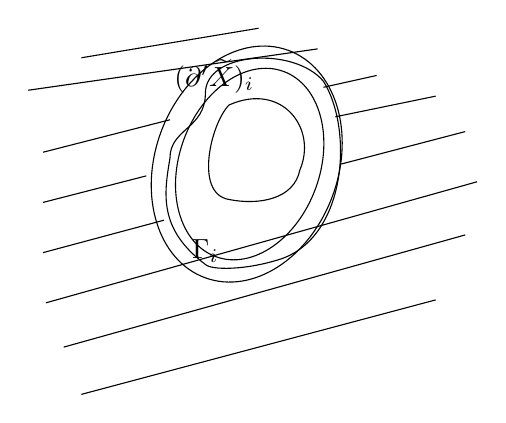
\begin{tikzpicture}[x=.75cm,y=.75cm]
\draw (-2,2.5)--(1,3) (-2.9,1.95)--(2,2.65);
\draw (-2.65,.9)--(-.5,1.45) (2.1,2)--(3.0,2.2);
\draw (-2.65,.05)--(-.9,.5) (2.3,1.5)--(4.0,1.85);
\draw (-2.65,-.8)--(-.6,-.25) (2.4,.7)--(4.5,1.25);
\draw (-2.6,-1.65)--(4.7,.4) (-2.3,-2.4)--(4.5,-.5) (-2,-3.2)--(4,-1.6);
\draw[rotate around={-20:(.8,.7)}] (.8,.7) ellipse (1.55 and 2.05);
\draw[rotate around={-20:(.85,.7)}] (.85,.7) ellipse (1.19 and 1.67);
\draw (.1,-1.0) .. controls (-.7,-.4) and (-.6,.2) .. (-.5,.8)
 .. controls (-.5,1.3) and (.1,1.3) .. (.1,1.9)
 .. controls (.1,2.6) and (1.6,2.7) .. (2.1,2.1)
 .. controls (2.6,1.3) and (2.5,-.5) .. (1.4,-.9)
 .. controls (.8,-1.1) and (.2,-1.1) .. (.1,-1.0);
\draw (.5,.1) .. controls (-.1,.2) and (.2,1.4) .. (.5,1.7)
 .. controls (1.4,2.1) and (2,1.3) .. (1.7,.6)
 .. controls (1.6,.1) and (1,.0) .. (.5,.1);
\node at (.25,2.18) {$(\partial'\widetilde X)_i$};
\node at (.1,-.77) {$\Gamma_i$};
\end{tikzpicture}}

\margin{C'est une composition
rétrécissage $\circ$ élargissage,
ou aussi élargissage $\circ$ rétrécissage.}

\deleted{\unsure{6)}} \uline{\unsure{Commutativité}} de l'opération
de panachage relative à diverses
composantes connexes de $K$.

6) Cas d'une composante \inserted{$C$} de $K$ boucle
isolée \inserted{plongée $\unsure{\mathbb R|\mathbf R}$-analytique}. L'opération de panachage revient
alors tjrs à une composition de 1°) enlever
une couronne \inserted{$\unsure{\mathbb R|\mathbf R}$-analytique}
autour de
$C$ 2°)
Recoller \inserted{$\unsure{\unsure{\mathbb R|\mathbf R}\text{-analytiquement}}$} par
un cylindre les deux
bords \inserted{qui restent} de la couronne
enlevée\ldots

\figure{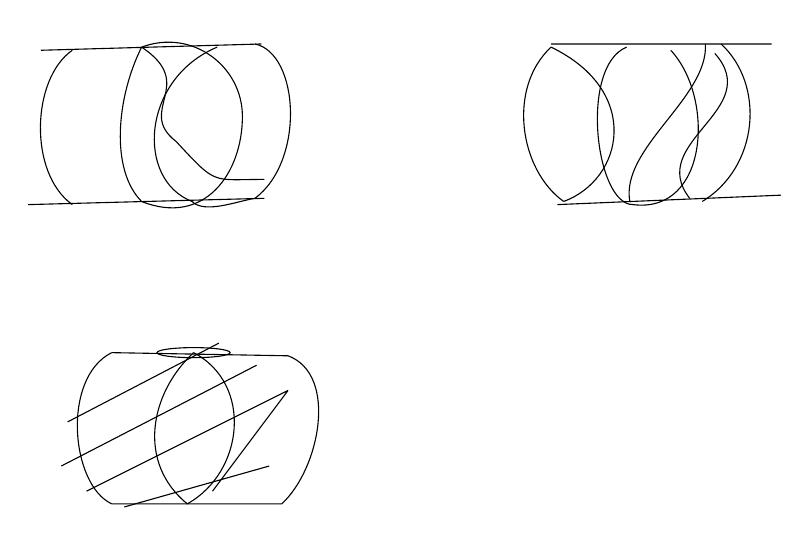
\begin{tikzpicture}[x=.8cm,y=.8cm]
\begin{scope}
\draw (-.4,1.25)--(3.1,1.35) (-.6,-1.2)--(3.15,-1.1);
\draw (.1,1.25) .. controls (-.55,.8) and (-.6,-.7) .. (.1,-1.2);
\draw (3,1.35) .. controls (3.7,1.2) and (3.8,-.5) .. (3,-1.1);
\draw (1.2,1.3) .. controls (.8,.5) and (.7,-.65) .. (1.2,-1.15)
 .. controls (2.2,-1.55) and (2.8,-.7) .. (2.8,.2)
 .. controls (2.8,1) and (2,1.6) .. (1.2,1.3);
\draw (1.2,1.3) .. controls (2.1,.7) and (1.1,.3) .. (1.75,-.2)
 .. controls (2.4,-.9) and (2.3,-.8) .. (3.15,-.8);
\draw (2.4,1.3) .. controls (1.2,.8) and (1.1,-.8) .. (2,-1.15)
 .. controls (2.2,-1.35) and (2.7,-1.15) .. (3,-1.1);
\end{scope}
\begin{scope}[xshift=6.4cm]
\draw (-.3,1.35)--(3.2,1.35) (-.2,-1.2)--(3.35,-1.05);
\draw (-.3,1.3) .. controls (-1.0,.65) and (-.8,-.65) .. (-.1,-1.15);
\draw (-.3,1.3) .. controls (1.15,.6) and (.85,-.8) .. (-.1,-1.15);
\draw (2.4,1.35) .. controls (3.1,.7) and (3,-.6) .. (2.1,-1.15);
\draw (.9,1.3) .. controls (.15,1) and (.4,-1.2) .. (1,-1.2)
 .. controls (2.2,-1.35) and (2.3,.5) .. (1.6,1.25);
\draw (2.15,1.35) .. controls (2.2,.5) and (.8,-.3) .. (.95,-1.15);
\draw (2.3,1.2) .. controls (3.1,.3) and (1.2,-.2) .. (1.9,-1.1);
\end{scope}
\begin{scope}[xshift=.5cm,yshift=-3.8cm]
\draw (.1,1.2)--(2.9,1.15) (.1,-1.2)--(2.8,-1.2);
\draw (.1,1.2) .. controls (-.7,.8) and (-.55,-.9) .. (.1,-1.2);
\draw (2.9,1.15) .. controls (3.7,.85) and (3.4,-.65) .. (2.8,-1.2);
\draw (1.4,1.2) ellipse (.58 and .08);
\draw (1.4,1.2) .. controls (.7,.55) and (.5,-.55) .. (1.3,-1.2)
 .. controls (2.2,-.7) and (2.35,.7) .. (1.4,1.2);
\draw (-.6,.1)--(1.8,1.35) (-.7,-.6)--(2.4,1.0)
 (-.3,-1.0)--(2.9,.6) (1.7,-1.0)--(2.9,.6)
 (.3,-1.25)--(2.6,-.6);
\end{scope}
\end{tikzpicture}}

relations avec les \deleted{\unsure{deux}} \inserted{\unsure{petits}} \unsure{plongements} conformes
d'une petite couronne\ldots
% archive foliation: 3
\scanpage{5}
7) Modules pour $S\subset K\subset X$

On suppose \inserted{\deleted{$X$} compact, et} pour simplifier $X$ \deleted{compact} \inserted{sans bord} orienté.
Ceci dit, on fixe $S_0\subset K_0\subset X_0$ situation
top, et on \uline{rigidifie} $(S\subset K\subset X)$ en
se donnant une classe d'isotopie d'homeo.
top. avec la situation standart. On élimine
ainsi les autos, sauf dans le cas
\deleted{$\unsure{K_0}$} où $X_0$ a des composantes de degré
$0,1$\ldots

Pour avoir un ``\unsure{nb} fini de modules'',
on \inserted{pourrait} exige\inserted{r} que les arêtes de $K$ soient
des arcs de cercle pour la conn.
projective canonique. Mais les
``cartes \inserted{coll.} holomorphes'' ne satisfont pas
néc. à cette condition ! On pourrait
exiger plutôt que pour \deleted{\unsure{nos}} les
paramétrisations géodésiques sur le
découpé, \unsure{ses composés|ses diagrammes} avec l'homéomorphisme
de recollage soient linéaires. [Éventuellement
on pourrait exiger l'équidistance \inserted{des sommets} \deleted{\unsure{sur}}
chaque composante connexe du bord de
le découpé\ldots] Mais on a des ennuis
pour les morceaux \deleted{de genre $0$} \inserted{qui sont des disques \unsure{non ponctués}}
: pas de métrique nat \unsure{const.}. Il
% archive foliation: 4
\scanpage{6}
% Drawings and formula blocks follow their positions in the supplied scan.
% Formula writing at the foot is upside down in the supplied scan.
\figure{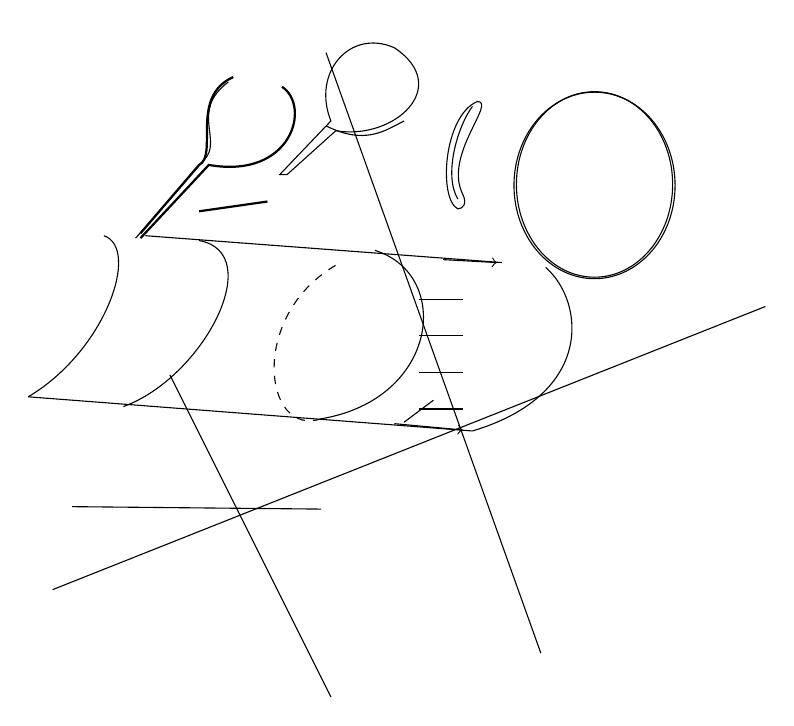
\begin{tikzpicture}[x=.62cm,y=.62cm]
\draw[thick] (1.2,3.5)--(2.4,4.9) .. controls (2.8,5.1) and (2.2,6.3) .. (3.1,6.7);
\draw[thick] (1.2,3.4)--(2.6,4.9) .. controls (4.3,4.6) and (4.7,6.1) .. (4.1,6.5);
\draw (1.1,3.4)--(2.5,5) .. controls (2.9,5.4) and (2.2,6) .. (3,6.6);
\draw[thick] (2.4,3.95)--(3.8,4.15);
\draw (4.05,4.7)--(5.1,5.8) .. controls (4.7,6.8) and (5.5,7.7) .. (6.4,7.3)
 .. controls (7.6,6.5) and (6.4,5.4) .. (5.2,5.6)--(4.2,4.7)--cycle;
\draw (5.0,5.7) .. controls (5.8,5.3) and (6.2,5.6) .. (6.6,5.8);
\draw (7.7,4.0) .. controls (7.3,4.2) and (7.4,5.9) .. (8.1,6.2)
 .. controls (8.5,6.2) and (7.4,5.1) .. (7.8,4.3) .. controls (7.9,4.1) and (7.8,4) .. (7.7,4);
\draw (7.7,4.2) .. controls (7.4,4.7) and (7.7,5.7) .. (8.0,6.1);
\draw (10.5,4.5) ellipse (1.6 and 1.9);
\draw (10.5,4.48) ellipse (1.65 and 1.91);
\draw (1.3,3.45)--(8.6,2.9) (-1.1,.15)--(8.0,-.55);
\draw (-1.1,.15) .. controls (.5,1.1) and (1.2,3.2) .. (.45,3.45);
\draw (.85,-.05) .. controls (2.5,.55) and (3.8,3.1) .. (2.4,3.35);
\draw (4.9,-.3) .. controls (7.3,.1) and (7.6,2.65) .. (6.0,3.15);
\draw[dashed] (4.9,-.3) .. controls (3.7,-.7) and (3.4,1.9) .. (5.3,2.9);
\draw (8,-.55) .. controls (10.5,.2) and (10.3,2.1) .. (9.5,2.8);
\foreach \y in {-.1,.65,1.4,2.15} {\draw (6.9,\y)--(7.8,\y);}
\draw[->] (7.4,2.96)--(8.5,2.9);
\draw[->] (6.4,-.4)--(7.8,-.53);
\draw (6.6,-.37)--(7.2,.08);
\draw (-.2,-2.1)--(4.9,-2.15);
\draw (-.6,-3.8)--(14,2.0);
\draw (5.0,7.2)--(9.4,-5.1) (1.8,.6)--(5.1,-6.0);
\end{tikzpicture}}

\[
\widetilde K_i\qquad
\unsure{\Sigma|\sum}(X_i,\partial X_i)=|\widetilde K_i|
\]

\margin{\[
|x'|,|y'|\leq\sqrt{x'^2+y'^2}\leq|x'|+|y'|
\]
\[
\int|x'|,\int|y'|\leq\int\unsure{-}\leq\int|x'|+\int|y'|
\]}

\figure{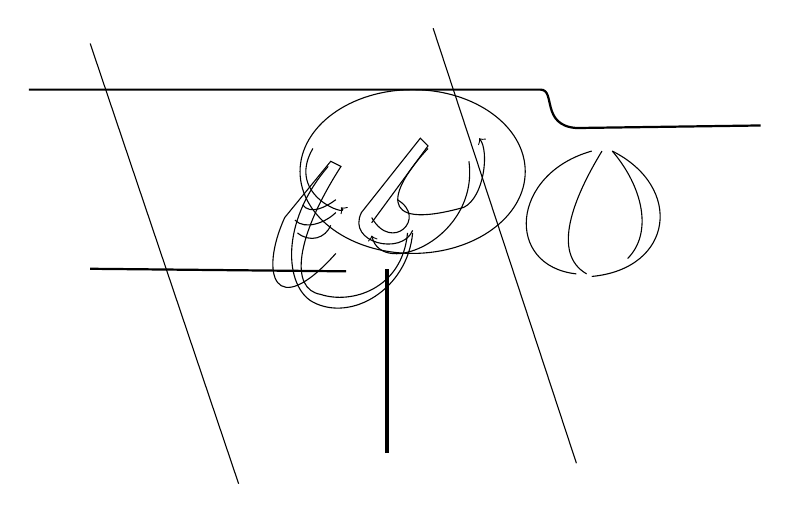
\begin{tikzpicture}[x=.65cm,y=.65cm]
\draw[thick] (-4,3.3)--(6,3.3) .. controls (6.3,3.3) and (6,2.6) .. (6.7,2.55)--(10.3,2.6);
\draw[thick] (-2.8,-.2)--(2.2,-.25);
\draw[very thick] (3,-3.8)--(3,-.2);
\draw (3.5,1.7) ellipse (2.2 and 1.6);
\draw[->] (1.55,2.15) .. controls (1,1.2) and (2.3,.8) .. (2.1,1.0);
\draw[->] (4.6,1.9) .. controls (4.8,.4) and (2.9,-.4) .. (2.7,.45);
\draw (2,.1) .. controls (.8,-1.25) and (.5,-.3) .. (1.0,.8)--(1.9,1.9)--(2.1,1.8)
 .. controls (1.2,.4) and (1.1,-.6) .. (1.7,-.7)
 .. controls (2.3,-.9) and (3.3,-.6) .. (3.4,.5);
\draw (1.85,1.8) .. controls (.9,.7) and (1.0,-.55) .. (1.55,-.85)
 .. controls (2.3,-1.25) and (3.4,-.6) .. (3.5,.5);
\draw (2.7,.7)--(3.8,2.2)--(3.65,2.35)--(2.5,.9)
 .. controls (2.2,.3) and (3.3,.05) .. (3.5,.55);
\draw[->] (3.8,2.15) .. controls (3.1,1.4) and (2.7,.5) .. (4.5,1.0)
 .. controls (4.9,1.2) and (5,2.1) .. (4.8,2.35);
\draw (2.7,.8) .. controls (3.1,.1) and (3.8,.8) .. (3.2,1.15);
\draw (1.25,.5) .. controls (1.5,.3) and (1.8,.4) .. (1.9,.65);
\draw (1.2,.75) .. controls (1.4,.55) and (1.8,.7) .. (2,.9);
\draw (1.35,1.05) .. controls (1.5,.85) and (1.8,1) .. (2.0,1.15);
\draw (7,2.1) .. controls (5.4,1.65) and (5.3,-.15) .. (6.7,-.3);
\draw (7.2,2.1) .. controls (6.65,1.2) and (6.2,.1) .. (6.9,-.3);
\draw (7.4,2.1) .. controls (8.8,1.4) and (8.6,-.2) .. (7,-.35);
\draw (7.4,2.1) .. controls (8,1.4) and (8.2,.5) .. (7.7,.0);
\draw (-2.8,4.2)--(.1,-4.4) (3.9,4.5)--(6.7,-4.0);
\end{tikzpicture}}

\[
\widetilde K=\varinjlim_{x\in K\setminus L}K_x,
\qquad K_x=\{y\in K\mid y\leq x\}
\]
\[
\left\{\begin{array}{l}
|\widetilde K|-|\widetilde L|\xrightarrow{\sim}|K|-|L|\\
(\widetilde K,\widetilde L)\text{ est ``pur''}
\end{array}\right.
\]

\diagram{\begin{tikzcd}[column sep=large,row sep=large]
\widetilde K \arrow[r,"\pi"] & K\ {\deleted{\unsure{\cup}}}\\
\widetilde L=\pi^{-1}(L) \arrow[u,phantom,"\cup",description] \arrow[r] & L \arrow[u,bend right=55]
\end{tikzcd}}

\deleted{$\widetilde L_0=\pi^{-1}(L_0)\subset\widetilde K_0$}

\deleted{$\widetilde L=T$}
% archive foliation: 5
\scanpage{7}
vaut mieux dès lors exiger que ces \unsure{sommes}
soient \uline{homographiques} par morceaux\ldots
Dans le premier cas (exiger que les
disques ds le découpé soient ponctués\ldots)
on trouve, en supposant $\unsure{\Pi|\pi}_0(K_0)\longrightarrow\unsure{\Pi|\pi}_0(X_0)$
surjectif, \deleted{et \unsure{qu'il n'y ait} pas de bouts isolés\ldots}
nb de modules \inserted{réels}
\[
N=\left(\sum_{\substack{f\in\unsure{\Pi|\pi}_0(X\setminus K)=F\\f\text{ pas \uline{un} disque}}}
(6g(f)+4\nu(f)\unsure{-}6)\right)+\deleted{\unsure{\mu}}
\]
\deleted{$\mu$ étant le nb de ``faces'' $f$
qui sont des \deleted{disques}\inserted{couronnes}.}

\margin{On suppose $X_0$ connexe
$K$ connexe
$\lambda$ la connexité
de $K$}
\inserted{$\unsure{N}$ à $g\geq2$}
\[
3g-3\qquad\text{où}\quad
2-2g=\unsure{\chi}=\sum_{f\in F}(2-2g(f)-\nu(f))
\inserted{+1-\lambda}
\]
\[
\text{i.e.}\quad 2g-2=\sum_{f\in F}(2g(f)-2+\nu(f))
+(\lambda-1)
\]
\[
g\unsure{-|=}1=\frac12\sum_{f\in F}[2g(f)-2+\nu(f)-1]
+\frac{\unsure{3|1}}2(\lambda-1)
\]
\[
\begin{aligned}
3(g-1)&=\frac32\sum_{f\in F}[2g(f)-2+\nu(f)]
+\frac32(\lambda-1)\\
&=\sum_{f\in F}\left[3(g(f)-1)+\frac32\unsure{\nu}(f)\right]
+\frac32(\lambda-1)
\end{aligned}
\]
\[
(g\geq2)\qquad
N\unsure{-|=}(\unsure{2|3}g-3)
=\sum_{\substack{f\in F\\f\text{ pas un disque}}}
\left(3g(f)+\frac{\unsure{5}}2\nu(f)-3\right)
+\deleted{\sum_{\substack{f\in F\\f\text{ disque}}}\unsure{(}}
\frac32(\mu+\unsure{1-\lambda})\overset{?}{\geq}0
\]
$\mu$ étant le nb de $f$ qui
sont des disques

\[
(g=1)\qquad N-1=\sum_{\substack{f\text{ pas un}\\\text{disque}}}
\bigl(\underbrace{4\nu(f)-6}_{\unsure{\geq}2}\bigr)-1
\]
[NB $g(f)=0$ tjrs]
% archive foliation: 6
\scanpage{8}
% Typed sheet is upside down in the scan; the two long diagonal cancellation strokes cross the list.
\deleted{
LISTE DE TERRAINS

\texttt{=====================}

\diagram{\begin{array}{ll}
\text{Réf. 2\quad LODEVE}&\text{2.450 M2 E.E.E. Expo. Est - vigne - route -}\\
&\text{Prix : 90.000 Frs}\\[4pt]
\text{Réf. 5 VERNAZOUBRES}&\text{4.750 M2 E.E.\quad Expo. Ouest - chêne - pin -}\\
&\text{route -\qquad Prix : 13.000 Frs}\\[4pt]
\text{Réf. 7 VERNAZOUBRES}&\text{161.640 M2 \uline{très isolé}\quad expo. Ouest - chemin}\\
&\text{Prix : 90.000 Frs}\\[4pt]
\text{Réf. 11 LE LEZ}&\text{5.000 M2 E.E.\quad expo. Sud - pinède -}\\
&\text{accès chemin Prix : 60.000 Frs}\\[4pt]
\text{Réf. 13 LACOSTE}&\text{11.000 M2 E.E.\quad Expo. Ouest - boisé -}\\
&\text{chemin\qquad Prix : 98.000 Frs}\\[4pt]
\text{Réf. 14 LACOSTE}&\text{13.390 M2 E.E.E. Expo. Sud - vigne - bois -}\\
&\text{Prix : 70.000 Frs}\\[4pt]
\text{Réf. 15 VERNAZOUBRES}&\text{23.000 M2 Source Expo. Ouest - boisé - Isolé -}\\
&\text{chemin\qquad Prix : 24.000 Frs}\\[4pt]
\text{Réf. 20 CAUX}&\text{Lotissement de 590 à 640 M2 entièrement terminé -}\\
&\text{Prix : 43.000 à 48.000\unsure{Nrs|Frs}}\\[4pt]
\text{Réf. 32 LACOSTE}&\text{1.000 M2 E.E.\quad Expo. Ouest - ancien jardin dans}\\
&\text{village\qquad Prix : 42.000 Frs -}\\[4pt]
\text{Réf. 33 FOZIERES}&\text{4.000 M2 E.E.\quad Expo. Est - boisé et arbres}\\
&\text{fruitiers - chemin - Prix 35.000 F}\\[4pt]
\text{Réf. 34 ARBORAS}&\text{22.500 M2 Beau point de vue - Expo. Ouest - vigne-}\\
&\text{2.500 M2 solde bois - chemin - Prix : 20.000 Frs}\\[4pt]
\text{Réf. 36 ARBORAS}&\text{4.000 M2 E.E. beau point de vue - expo. Ouest -}\\
&\text{chemin - oliviers - Prix : 26.000F}\\[4pt]
\text{Réf. 55 ST ETIENNE G.}&\text{6.000 M2 Elect. Expo. Sud - boisé - accès par deux}\\
&\text{chemins\qquad Prix : 40.000 Frs}\\[4pt]
\text{Réf. 57 VILLENEUVETTE}&\text{15.000 M2 E.E. Téléph. Expo. Est - ancienne vigne-}\\
&\text{chemin -\qquad Prix : 70.000 Frs}\\[4pt]
\text{Réf. 65 ST ETIENNE G.}&\text{5.000 M2 E.E. Expo. Est - jolie vue s/village -}\\
&\text{Prix : 50.000 Frs}\\[4pt]
\text{Réf. 69 ST ETIENNE G.}&\text{7.141 M2 E.E. Expo. Ouest - oliviers - vigne -}\\
&\text{chemin\qquad Prix : 35.000 Frs}
\end{array}}

.../...
}
% archive foliation: 7
\scanpage{9}
\textcircled{1} courbe ell. $\unsure{A|X}$ + géod. fermée \uline{orientée} $\sigma$

\textcircled{2} \deleted{Courbe}. \inserted{\unsure{grpe}} elliptique $X_0$
+ \deleted{\unsure{un sous}\ \illegible{1}} \inserted{\deleted{\unsure{de rang 1}}}
\deleted{$\unsure{\mathbb U}$}\inserted{$X_0(\mathbb C)$}

$+\unsure{\mathbb U_0}$-torseur $\sigma$

\textcircled{\unsure{3}} $X_0+\unsure{a}\in\unsure{H_1|\pi_1}(X_0)+\Gamma$
\inserted{\unsure{primitif}}

\textcircled{4}
Torseur $\Gamma$ \unsure{en} $\mathbb U$, et
\diagram{\begin{tikzcd}[column sep=small,row sep=small]
Z \arrow[r,phantom,"\underset{\text{discret}}{\subset}"] \arrow[d,phantom,"\simeq" rotate=90] & \mathbb C^*\\
\mathbb Z &
\end{tikzcd}}

\textcircled{5}

\textcircled{6}
% archive foliation: 8
\scanpage{10}
% Envelope recto; text is read after a clockwise quarter-turn.
UNIVERSITE DES SCIENCES ET TECHNIQUES
DU LANGUEDOC

\figure{\begin{tikzpicture}\draw (0,0)--(1,0);\end{tikzpicture}}

INSTITUT DE MATHEMATIQUES

Place Eugène Bataillon

34060 MONTPELLIER CEDEX

M. Grothendieck

\figure{\begin{tikzpicture}[x=.8cm,y=.8cm]
\draw (-.3,-1.1) .. controls (-1.4,-1.1) and (-1.8,.0) .. (-1.2,1)
 .. controls (-.9,1.4) and (-.4,1.7) .. (0,1.8)
 .. controls (1,1.65) and (1.6,.9) .. (1.5,.1)
 .. controls (1.5,-.8) and (.8,-1.2) .. (.2,-1.1);
\draw (.05,.2) .. controls (-.4,.4) and (-.25,1.15) .. (.05,1.2)
 .. controls (1.1,1.45) and (1.2,.3) .. (.6,.2)--cycle;
\fill (.66,.96) circle (.075);
\draw (.42,.81)--(.51,.81) (.465,.765)--(.465,.855);
\draw[line width=1.2pt] (-1.12,-.05) circle (.13);
\fill (-1.12,-.05) circle (.045);
\draw[line width=1.2pt] (.1,-.65) circle (.19);
\fill (.1,-.65) circle (.035);
\draw (6.7,2.2) .. controls (5.6,2.6) and (5.5,1.1) .. (5.2,.4)
 .. controls (5.1,-.1) and (5.3,-.5) .. (5.7,-.6)
 .. controls (6.7,-.3) and (7.0,.2) .. (7,.75);
\fill (6.65,.86) circle (.045);
\end{tikzpicture}}
% archive foliation: 9
\scanpage{11}
\textcircled{1} courbe elliptique $X$ + géod. fermée \uline{orientée} $\bar\Gamma$ \unsure{m.l. tr.}

\textcircled{2} --- $X$ + \deleted{\unsure{un groupe}} \unsure{plgt} \deleted{\unsure{un}} $\mathbb U$ (tore cpt standard) $\subset X_0$

\textcircled{3} --- $X$ + $a\in\unsure{\Pi|\pi}_1(X)$ élément \uline{primitif}

\textcircled{4} Ss. gpe discret $(\simeq\mathbb Z)$ \deleted{$Z\subset\mathbb C^*$}\inserted{$Z\subset\mathbb C^*\ (\Leftrightarrow b\in\mathbb C^*,\ 0<|b|<1)$}, et torseur $\Delta$ sous $\mathbb C^*$ \deleted{et $Z\subset\mathbb C^*$ discret}

\textcircled{5} Droite vectorielle \unsure{cxe} $E$, \deleted{(\unsure{NB} $\Delta=E^*$), et} \deleted{$\unsure{\{b,b^{-1}\}}$}\inserted{$b$} et $b\in\mathbb C\quad 0<|b|<1$

(\uline{NB} $\Delta=E^*$, \deleted{$Z$} $T=\mathbb C^*_{\unsure{m}},\quad Z=$ gpe engendré (par $b$)
\[
P=\widehat E,\quad \{u,u^{-1}\}=\deleted{\{b,b^{-1}\}}\{\unsure{hom.}\ b,b^{-1}\}
\]

\textcircled{6} \deleted{Forme $G$ de $\mathrm{GP}(1)_{\mathbb C}$}, + \deleted{élément $b\in$}\inserted{couple de Killing} \deleted{Borel}\inserted{$T\subset$} $B\subset G$ \deleted{, et $b\in B$ tel que} \inserted{$G$ déduit}
\deleted{le groupe $b$}
de $\mathrm{GP}(1)_{\mathbb C}$ en tordant (par un torseur sous $T$\inserted{$\simeq$ \unsure{(cas choisi)} (i.e. torseur sous $\mathbb C^*$)}
[qui ne \unsure{sera autre} que $E^*$] en posant $Z\in\deleted{\unsure{T}}\mathbb C^*=T(\mathbb C)$ groupe discret,
(i.e. $Z$ donné par $b$) $///\quad G\supset B\ni b$, avec $b$ $\frac12$ simple
et $|b|$ (défini \unsure{ind. près qu'à l'inverse}) $\ne1$

\[
\underset{\text{\textcircled{1}}}{\deleted{\mathrm{ens}}\{\Gamma\}}
\simeq\underset{\text{\textcircled{1}}}{X/\Gamma_0}
\simeq\underset{\text{\textcircled{$\unsure{3\prime|3}$}}}{\deleted{X/\unsure{\mathbb Z\mathbb R|\mathbb Z_{\mathbb R}}}}
\simeq\underset{\text{\textcircled{4}}}{\deleted{\Delta/\unsure{T_{\mathbb R c}}}}
\inserted{\deleted{\unsure{\text{gpe projectif réel}}}},\quad
\Delta/(T_c\cdot Z)\simeq
\]
\deleted{droite projective $P$}
ens des \uline{cercles} de $P$ \deleted{admettant} admettant \unsure{Fix} $(u,u^{-1})$ comme \unsure{bicentres} \textcircled{5}
% archive foliation: 10
\scanpage{12}
\begin{center}
UNIVERSITE DES SCIENCES ET TECHNIQUES\\
DU LANGUEDOC\\
\rule{0.7cm}{0.2pt}\\
INSTITUT DE MATHEMATIQUES\\
Place Eugène Bataillon\\
34060 MONTPELLIER CEDEX
\end{center}

Jean Pierre \unsure{Drij}
% archive foliation: 11
\scanpage{13}
\figure{
\begin{tikzpicture}\draw[red,line width=2pt] (0,0)--(12,.16)..controls(12.15,.2)and(12.15,.1)..(11.9,.1);\draw[blue!60!black,line width=2pt] (0,-.22)--(12,-.04)..controls(11.7,-.02)and(11.85,.1)..(11.95,.13);\fill[blue!60!black] (2.5,-.28) circle (.035);\end{tikzpicture}}
\deleted{\unsure{corps de base} $\mathbb C$}

\diagram{\begin{tikzcd}[column sep=small,row sep=large]
\text{\textcircled{1}}\arrow[d,Leftrightarrow] & \parbox{12cm}{courbe elliptique $X$ + géodésique fermée $\Gamma$/mod translations}\\
\text{\textcircled{2}}\arrow[d,Leftrightarrow] & \parbox{12cm}{courbe elliptique $X$ + \deleted{géodésique \unsure{fermée}}\inserted{\deleted{\unsure{ss. gpe à 1 dim.}}} sous-tore réel $\Gamma_0$ de la courbe elliptique des $X_0$ translations}\\
\text{\textcircled{3}}\arrow[d,Leftrightarrow] & \parbox{12cm}{courbe elliptique $X$ + \deleted{\unsure{générateur} primitif de}\inserted{sous-gpe \unsure{facteur} de rg $1\ Z\subset$} $\unsure{\Pi|\pi}_1(X)$}\\
\text{\textcircled{4}}\arrow[d,Leftrightarrow] & \parbox{12cm}{forme\inserted{\deleted{$\unsure{\Delta}$}$T$} de $G_m$, ($Z\subset T(\mathbb C)$\inserted{sous-gpe \deleted{discret}\inserted{libre} de rg $1$} \deleted{\unsure{avec} $|b|\ne1$}, et torseur $\Delta$ sous $T$\par
\textcircled{$4'$} forme $T$ de $G_m$, \deleted{et $\unsure{u}\in T(\mathbb C)-\unsure{\{\pm1\}}$}\inserted{$b\in\mathbb C\quad 0<|b|<1$} et torseur $\Delta$ sous $T$\inserted{couple $\{u,u^{-1}\}$}}\\
\text{\textcircled{5}}\arrow[d,Leftrightarrow] & \parbox{12cm}{droite projective $P$, + (autom. $u$ de $P$ non paraboliques (i.e. ayant $2$ pts fixes distincts) et ayant des val. propres $\lambda,\lambda^{-1}$ tels que $|\lambda|\ne1$ \unsure{CNS}, quitte à \deleted{\unsure{choisir}}\inserted{\unsure{permuter}} $\lambda,\lambda^{-1}$ \deleted{\unsure{condition}} que $|\lambda|>1$)}\\
\text{\textcircled{6}} & \parbox{12cm}{forme\inserted{$G$} de $\mathrm{GP}(1)_{\mathbb C}$, + ss-gpe discret $(\simeq\mathbb Z)$ $Z\subset\deleted{\mathrm{GP}(1)(\mathbb C)}\inserted{\unsure{G}}$ non unipotent (i.e. formé d'él. $\frac12$ simples, i.e. $\subset$ tore maximal $T$)}
\end{tikzcd}}

\[
\underset{\text{\textcircled{1}}}{\mathrm{or.\,comp}\{\Gamma\}}\simeq
\underset{\text{\textcircled{2}}}{\mathrm{or}(\Gamma_0)}\simeq
\underset{\text{\textcircled{3}}}{\mathrm{g\acute en}(Z)}\simeq
\underset{\text{\textcircled{$3'$}}}{\mathrm{g\acute en}(Z)}\simeq
\underset{\text{\textcircled{4}}}{\mathrm{Triv}(T)}
\]
\margin{$\simeq\underset{\text{\textcircled{5}}}{\mathrm{Fix}(u)}\simeq\underset{\text{\textcircled{6}}}{\mathrm{Bor}(\unsure{G|B}\supset Z)}$}

\textcircled{\unsure{$7'$}} Vect. complexe $V$ de rg $1$ + (réseau $\unsure{\Pi|\pi}$) + $(Z\subset\unsure{\Pi|\pi})$\inserted{fact. direct rg $1$} + torseur $X$ sous $V/\unsure{\Pi|\pi}$

\margin{\begin{tabular}{l}
Jun-Ichi Yamashita\\
c/o Mr. Mizuno,\\
43 Myoken-ch\=o, Showa-ku\\
Nagoya 466, JAPAN
\end{tabular}}
\figure{
\begin{tikzpicture}\draw[blue!60!black,line width=2pt] (0,0)--(12,0);\draw[red,line width=2pt] (0,-.2)--(12,-.2);\end{tikzpicture}}
% archive foliation: 12
\scanpage{14}
\figure{
\begin{tikzpicture}[x=0.65cm,y=0.65cm]
\draw[red,line width=2pt,rounded corners=2pt] (0,0) rectangle (16,11);
\draw[blue,line width=2pt,rounded corners=2pt] (.2,.2) rectangle (15.8,10.8);
\end{tikzpicture}}

\figure{
\begin{tikzpicture}[x=0.7cm,y=0.7cm]
\node[align=left,anchor=west] at (0,2.6) {of\\Science};
\draw[red] (0,.7)--(.2,1.1)--(.9,.95)..controls (1.7,1.2) and (2.05,2.1)..(2.2,3)--(2.6,3.1)..controls (3,2.3) and (2.4,1.3)..(1.7,.65)--(.1,.6)--(0,.7);
\draw[red] (0,.55)--(.8,.55)--(.9,.35)--(0,.35);
\draw[red] (1.6,.65)--(2.9,1.2)--(3.3,.75)--(2,.55);
\draw[red] (1.6,.8)--(2.9,1.35) (1.75,.7)--(3.1,1.03) (1.8,.55)--(3.3,.78);
\draw[red] (2.2,3)--(2.05,3.55) (2.3,3)--(2.3,3.6) (2.4,3)--(2.55,3.6) (2.55,3.05)--(2.8,3.55);
\foreach \x/\y in {1/.8,1.3/.9,1.6/1,1.9/1.2,2.1/1.4,2.3/1.6,2.4/1.9,2.5/2.2,2.4/2.5,2.4/2.8,1.4/.65,1.7/.75,2/1,2.2/1.2,2.5/1.5,2.6/1.8,2.6/2.1,2.6/2.4,2.6/2.7} {\draw[red] (\x,\y) circle (.06);}
\node at (1.7,0) {NAGOYA UNIV.};
\end{tikzpicture}}
% crop-candidate: scan 14

\figure{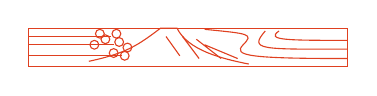
\begin{tikzpicture}[x=.7cm,y=.7cm]
\draw[red!50!brown] (0,0) rectangle (5.8,.7);
\draw[red!50!brown] (0,.2)--(1.7,.2) (0,.4)--(1.55,.4) (0,.55)--(1.5,.55);
\draw[red!50!brown] (1.1,.1)..controls(1.8,.25)and(2,.4)..(2.4,.7)--(2.7,.7)..controls(2.9,.3)and(3.5,.15)..(4,.05);
\draw[red!50!brown] (2.5,.55)--(2.75,.2) (2.8,.55)--(3.1,.15) (3.05,.5)--(3.5,.15) (3.2,.4)--(3.8,.15);
\draw[red!50!brown] (3.2,.68)..controls(4,.6)and(4.1,.6)..(3.9,.4)..controls(3.7,.2)and(4,.15)..(5.8,.15);
\draw[red!50!brown] (4.3,.65)..controls(4,.3)and(4.2,.32)..(5.8,.32);
\draw[red!50!brown] (4.55,.65)..controls(4.3,.48)and(4.7,.48)..(5.8,.48);
\foreach \x/\y in {1.2/.4,1.4/.5,1.65/.45,1.8/.35,1.55/.25,1.75/.2,1.3/.6,1.6/.6} {\draw[red!50!brown] (\x,\y) circle (.08);}
\end{tikzpicture}}
% crop-candidate: scan 14

\diagram{\begin{array}{|c|c|c|}\hline
& & \text{\unsure{日本郵便}}\\\hline
20.12.77&\begin{gathered}\text{名古屋大学内}\\\text{NAGOYA DAIGAKUNAI}\\\text{JAPAN}\end{gathered}&0,340\\\hline
\end{array}}
HI208

Professeur Alexandre Grothendieck

34700 Villecun (Lodève)

\uline{FRANCE}

VIA AIR MAIL\\
PAR AVION

\diagram{\begin{array}{|c|}\hline
\text{PAR AVION}\\
\text{航空郵便}\\\hline
\end{array}}

\margin{\unsure{340}}

$\{\lambda,\lambda^{-1}\}\qquad |\lambda|\ne1$

$\lambda+\lambda^{-1}=\alpha\qquad\deleted{\unsure{ssi}}\quad\alpha\notin[-2,+2]$

$\alpha^2-4$

$\unsure{\Leftrightarrow}\lambda\bar\lambda=1$\\
$\bar\lambda=\lambda^{-1}$\\
$\lambda+\lambda^{-1}$ \uline{réel}

Donc $\lambda\ne\lambda^{-1}$ i.e. $\lambda^2\ne1$ i.e. $\lambda\ne\pm1$ i.e. $\alpha\ne\pm2$
% archive foliation: 13
\scanpage{16}
\mspage{1}
\begin{flushright}Les Aumettes 15.4.1984\end{flushright}

Dear Lipman Bers,

Together with Yves Ladegaillerie (a former student of mine) we are running a microseminar on the Teichmüller spaces and groups, my own motivations coming mainly from algebraic geometry, and Ladegaillerie's from his interest in the topology of surfaces. Lately we have met with a problem which I would like to submit to you, as I understand you are the \unsure{main} expert on Thurston's hyperbolic geometry approach to Teichmüller space. Before stating the specific problem on hyperbolic ``pants'' (which things boil down to), let me tell you what we are really after.

Assuming given a compact oriented surface with boundary $X_o$ \deleted{\unsure{now}} as a reference-surface for constructing the Teichmüller-type spaces, of genus $g$ and with \hspace{0.5cm} ``holes'' (satisfying $2g-2+\nu>0$), my primary interest is in the more ``algebraic'' version of Teichmüller space, corresponding to the question of classifying algebraic non singular curves over $\underline{C}$, of genus $g$, with a system of \hspace{0.5cm} points (all distinct) given on $X$, together with a ``Teichmüller rigidification'' of $(X,S)$ namely a homotopy equivalence between $X_o$ and $X\backslash S$. I'll denote this space, homeomorphic to $\underline{C}^{d}$ (where $d=3g-3+\nu$), by $\widetilde M_{g,\nu}$ (the tilda suggesting that it is the universal covering of a finer object I am still more interested in, namely the algebraic variety (or rather ``multiplicity'', or ``stack'' in the terminology of Mumford-Deligne) of \unsure{moduli} for algebraic curves of type $(g,\nu)$.
Thurston however considers a different modular space, where algebraic curves with a given system of points are replaced by compact conformal oriented surfaces \uline{with boundary}, giving rise to a modular space $\widetilde{MB}_{g,\nu}$ (where the letter B recalls that we are classifying structures with boundary) homeomorphic to $\underline{C}^{d}\mathbin{\mathrm{x}}(\underline{R}^{\unsure{\mathrm{x}|*}+})^{\nu}$, where the extra factor \deleted{$\unsure{\underline C^d}$} corresponds to the extra parameters introducing through the existence of the boundary, namely the length's of the \deleted{\unsure{various}} components of the boundary with respect to the canonical hyperbolic structure on the given surface. Our interest is in pinpointing the precise relationship between the two modular spaces. The obvious idea here is to consider the case of an algebraic curve with $\nu$ points given as a limit-case of a \inserted{compact} conformal surface with boundary, when all the lengths $\ell_i$ of the components of the boundary tend to zero. Therefore, it looks suitable to consider both modular spaces above as imbedded in a larger third one, which corresponds to the same modular problem as in Thurston's theory, except that we allow the ``boundary'' to have some components reduced to just one point, in the neighbourhood of which $X$ is just a conformal surface without boundary, but with a given point
% archive foliation: 15
\scanpage{17}
\mspage{2}
(viewed as a component of such a ``generalised boundary''). We now should \deleted{should} get a modular space for ``compact conformal oriented surfaces with generalized boundary'' (of type $g,\nu$ and rigidified via $X_o$), call it $\widetilde{MB}_{g,\nu}$, homeomorphic to $\underline C^d\mathbin{\mathrm{x}}(\underline R^{\deleted{*}+})^{\nu}$, where now the second factor corresponds to \deleted{\unsure{the}} the ``parameters'' $\ell_i$, which are allowed to take also value $0$ (which means that the corresponding component of the generalized boundary is just one point). Thus $\widetilde{MB}_{g,\nu}$ appears as a variety with boundary (in the topological sense - in the real analytic sense, the ``boundary'' admits ``corner-like'' points obviously), and $\widetilde M_{g,\nu}$ appears as a part of the boundary.

My interest is in a better geometric understanding of the situation, which should be ``intrinsic'' namely not depend on any particular choice of a surgical decomposition of the reference surface $X_o$ into ``pants'', used in order to describe in a handy way \unsure{the} standard ``coordinate\deleted{\unsure{s}}functions'' on the modular space $\widetilde{MB}_{g,\nu}$. There appears to be a geometrically meaningful retraction of $\widetilde{MB}_{g,\nu}\deleted{\unsure{\nu}}$ upon $\widetilde M_{g,\nu}$ (commuting to the operations of the Teichmüller modular group), the fibers being homeomorphic to $(\underline R^+)^{\unsure{\nu}}$ - more specifically, I expect the semi-group $(\underline R^+)^I$ (where I is the set of indices for the ``holes'' of $X_o$) to act on $MB$ in a natural way, with free action of the subgroup $(R^{+*})^{\nu}$ upon $\widetilde{MB}^{o}$, in such a way that $\widetilde M$ is just the quotient of $\widetilde{MB}$ by this action (or of $\widetilde{MB}^{o}$ by the action of the \deleted{\unsure{unit-g}} corresponding subgroup), and that each fiber\inserted{$F$} is isomorphic to $(\underline R^+)^I$ by the choice of any ``origin'' in $F\cap\widetilde{MB}^{o}$.

Of course, ``\unsure{computionally}'', in terms of a decomposition of $X_o$ into pants, the idea of such an operation is pretty obvious - namely letting the components $\lambda_i$ of $\lambda\in(\underline R^+)^I$ act as a ``multiplier'' on the corresp\inserted{ond}ing coordinate $\ell_i$. However, it is not clear that this operation is intrinsic - and if it were intrinsic, an intrinsic geometric description would still be \deleted{\unsure{to}} desired.

Of course, in the description of the situation proposed above, the retraction of $\widetilde{MB}$ upon $\widetilde M$ is obtained by multiplying with the $0$ multiplier (all $\lambda_i$ are $0$). Now there is a direct geometrical description of \deleted{this} a retraction, by hyperbolic surgery. Namely, for any \inserted{compact} conformal surface of type $g,\nu$ with generalized boundary, let's ``fill in'' the holes which correspond to ordinary components of the boundary, which are riemannian oriented circles, by ``gluing in'' the cones on these circles (which are canonically endowed with a conformal structure, using the riemannian structure on the given circles). Thus we get a ``functor'' from \inserted{compact} conformal surfaces with generalized boundary (of type $g,\nu$) to compact conformal surfaces \uline{without boundary}, endowed with a system of $\nu$ points (making up a
% archive foliation: 16
\scanpage{18}
\mspage{3}
``wholly degenerate'' generalized boundary). When we throw in the rigidifications and go over to isomorphism classes, this should give the desired retraction. However, the geometric situation is a lot richer still, as the compact surface without boundary obtained through surgery is endowed, not only with a system of $\nu$ points, but moreover with a system of mutually disjoint \uline{discs} around these points. The shape of these discs is by no means arbitrary - we'll say that a system of discs around $\nu$ points on a compact \inserted{conformal} surface $X^{\wedge}$ without boundary is ``admissible'', if the situation can be obtained as above (up to isomorphism) from surgery, starting with a compact conformal surface $X$ with boundary. (NB Among the given ``discs'', we should allow that some should be reduced to their center - we'll call them ``degenerate''.) The condition of admissibility can be expressed intrinsically, by stating that \deleted{the} for every non-degenerate component $\Gamma_i$ of the system of boundaries of those discs, the two operations we got of the standard circle group (of complex numbers of module $1$) upon $\Gamma_i$, by using the fact that it is (on the one hand) the boundary of the disc $D_i$, and (on the other hand) that it is a component of the boundary of the hyperbolic surface $X^{\wedge}\backslash(\bigcup_j D_j^{o})$, should be the same. When $X^{\wedge}$ and the points $s_i$ on $X^{\wedge}$ are given, the possible \inserted{admissible} systems of discs around the points $s_i$ depend on $\nu$ parameters - and the first idea which flips to mind to give a more precise meaning to these ``parameters'', is to view them as being the ``radii'' of those discs. But then we'll have to define what we mean by these !
\margin{!}

The idea here is that, when we have a conformal disc $D$ and an \unsure{interior} point $s$ of $D$, then $D$ may be viewed as canonically embedded in \unsure{the} tangent space $T_s$ to $D$ at $s$, as the ``unit disc'' at $s$. Thus, in the situation above of an\deleted{\unsure{just}} admissible system of discs $(D_i)_{i\in I}$ around $(s_i)_{i\in I}$, for every $s_i$ corresponding to a non-degenerate $D_i$, we get a canonical disc
\[
\Delta_i\subset T_{s_i}
\]
in the tangent space - and of course, for degenerate $D_i$, we'll take $\Delta_i$ to be degenerate too. The discs we get in a\deleted{\unsure{y}} given $T_{s_i}$ (for a fixed system $(s_i)$, and a variable \inserted{admissible} system of discs around these $s_i$) are all discs in the strict euclidean sense, given by an unequality
\[
|z|\le r_i\ ,
\]
where $z\mapsto|z|$ denotes some hermitian metric on $T_{s_i}$ compatible with the conformal structure - this metric being \deleted{defined}\inserted{unique} up to a scalar factor. the set\inserted{$R_i$} of all those possible discs (the non-degenerate ones\deleted{\unsure{,}} say) may be viewed in a natural way as a ``torsor'' (= principal homogeneous space)
% archive foliation: 17
\scanpage{19}
\mspage{4}
\unsure{uncer|under} $\underline R^{+*}$, which plays here the role of the parameter space of \inserted{all} possible (non degenerate) ``radii'' at $s_i$. If we admit also radius zero, we accordingly get a parameter space $R_i^{\wedge}$, which may be viewed as a torsor of sorts \unsure{under} $\underline R^+$. Thus the set of radii for a given admissible system of discs $D_i$ around the points $s_i$ may be viewed as a point of the product-space
\[
r=(r_i)_{i\in I}\in R^{\wedge}=\prod_{i\in I}R_i^{\wedge}\ .
\]
My expectation is that an admissible set of discs $(D_i)$ is well determined by the knowledge of the corresponding set\inserted{$r$} of radii \deleted{$\unsure{r}$}, and moreover that a given set\inserted{$r$} of radii \deleted{$\unsure{r}$} corresponds to \deleted{\unsure{a}}\inserted{an admissible} system of \deleted{admissible} discs iff it satisfies a set of unequalities
\[
r_i<\rho_i\ ,
\]
where
\[
\rho=(\rho_i)_{i\in I}\in R=\prod_{i\in I}R_i
\]
is a \inserted{some} fixed system of radii, corresponding to a fixed system of choices of hermitian metrics in the tangent spaces $T_{s_i}$.

I now see that this ``expectation'' does'nt quite match\inserted{with} the previous one, about a ``natural operation'' of $(\underline R^{\unsure{+*|+}})^I$ upon $\widetilde{MB}$, having certain properties - it would match only if all $\rho_i$ where equal to $+\infty$ (hence not in $R_i$ itself strictly speaking). I must confess I did'nt look too thoroughly yet at the situation, and moreover I've been busy with rather different kind of things for the last two or three months, and lost\inserted{contact} a little\ldots\ \deleted{contact.} What is clear however is that the main key to an understanding of the general situation, is in an understanding of the basic particular case of Thurston's pants. If we number $0,1,\infty$ the three ``holes'' of such a pant, the surface $X^{\wedge}$ can be identified canonically to the Riemann sphere, and the basic question then is to understand how the pant is imbedded in this sphere $\Sigma$, as a complement of \deleted{(open)} the union of (open) discs around the points $0,1,\infty$, these discs forming an ``admissible system''. So the main question is about understanding the structure of all possible admissible systems of three discs on $\Sigma$.

\unsure{Pyzzling|Puzzling} a little about this problem, the following model came to my mind (corresponding to ``limiting radii'' $\rho_i$ which are \uline{finite}, not infinite). I view $\Sigma$ as endowed with it's usual euclidean metric, for which the real projective line is a great circle, with $0,1,\infty$ at equal distance from each other on this equator. These points may be viewed as the centers of three ``orange \deleted{quarters}\inserted{slices}'', making up a cellular subdivision of $\Sigma$, where the common boundary of two among the ``\deleted{quarters}\inserted{slices}'' $Q_i$ ($i\in\{\unsure{C|0},1,\infty\}$) is a half-great circle passing in between $s_i$ and $s_j$ at equal
% archive foliation: 18
\scanpage{20}
\mspage{5}
distance from both, these three half-circles joining at the two poles $P^+$ and $P^-$. The ``disc'' $Q_i$ around $s_i$ has a conical structure around $s_i$ (as has any conformal pointed disc), and we may take the concentric \deleted{\unsure{discs}} discs $\lambda_iQ_i$ with
\deleted{$\unsure{i}$}
\[
0<\lambda_i<1\ .
\]
The model I had in mind was that the (non degenerate) admissible systems of discs around the points $s_i$ ($i\in\{0,1,\infty\}$) \unsure{were} exactly the systems of discs $\lambda_iQ_i$, with $\lambda_i$ as above. (If we allow some discs to be degenerate, this means that instead of the unequality above we merely demand $0\le\lambda_i<1$, $0$ not excluded.)

This model, if correct, would give a rather precise description of the inclusion relationships between pants, when these are considered as embedded in the sphere. The intersection of all would be this system of three half circles $C_i$, and the two poles $P^+,P^-$ would play a significant role in the \unsure{geometry} of the pants, from this point of view. But it does'nt seem that neither those half circles (which need not be geodesical I guess), nor the two poles, have ever been described as intrinsically associated to a pant. Of course, this model would give alternative ``parameters'' $\lambda_i$ for describing a pant, which are best suited for grasping the pants in terms of spherical geometry. The next question would be an understanding of the relationship between these parameters, and Thurston's $\ell_i$. Maybe it is unreasonable to expect that for given index $i\in\{0,1,\infty\}$, the length $\ell_i$ depends only on $\lambda_i$ and not on the other parameters $\lambda_j$ - and for this reason, \deleted{\unsure{the}} the intuition at the beginning of this letter, using Thurston's coordinate functions and notably the $\ell_i$'s to get a fibration structure on $\widetilde{MB}$ over $\widetilde M$, in terms of a given decomposition of $X_o$ into pants, is probably not really relevant, namely it is non intrinsic. Assuming the model I am suggesting is correct, the accurate description \deleted{\unsure{but}} of $\widetilde{MB}$ in terms of $\widetilde M$ would be
\[
\widetilde{MB}\simeq\widetilde M\mathbin{\mathrm{x}}[0,1[^I\ ,
\]
where the second factor on the right hand sight refers to the system of multipliers $\lambda_i$ ($i\in I$), tied to the $r_i$ above by $r_i=\lambda_i\rho_i$.

My question of course is whether you have any information or idea to propose, especially on the basic problem of relying pants to spherical geometry, and more specifically, whether the model above is likely to hold, or is definitely false. Also, one difficulty we found with hyperbolic geometry of conformal surfaces,\inserted{is} that apart from existence and unicity of the hyperbolic structure (compatible with the given conformal one and for which the boundary is geodesic), there seems to be little
% archive foliation: 19
\scanpage{21}
\mspage{6}
hold on more specific properties. As an example, starting with a \inserted{compact} conformal surface with boundary $X$ (a pant, say), of hyperbolic type, and removing an (open) ``collar'' around the bou\inserted{n}dary, we get another surface with boundary $X'$- what about the relation \deleted{\unsure{of}}\inserted{between} the two corresponding metrics ? Assuming the model for pants above is correct, it would be nice to have an explicit expression of the metric of a pant in terms of the parameters $\lambda_i$,

With my thanks for your attention, and for \unsure{whetever|whatever} comment you will care to make, very sincerely \unsure{ypur's|your's}
% archive foliation: 20
\scanpage{24}
Métriques canoniques\\
sur surfaces conformes

\figure{\begin{tikzpicture}\draw (0,.08)..controls (.08,-.05) and (.34,-.05)..(.45,.12);\end{tikzpicture}}
% archive foliation: 26
\scanpage{25}
a) deux \unsure{réellifications|réalifications} de types opposés compatibles,\\
i.e. un couple compatible d'antipodisme et inversion

b) \unsure{Métrique|Métriques} \unsure{sphérique|sphériques} + grand cercle

c) cercle + structure torique compatible dessus,\\
i.e. antiinvolution \deleted{\unsure{de points fixes}}\inserted{sans pts fixes},\\
et paire de points conjugués par\\
\unsure{la dite}

d) Tore compact $T\subset G=\operatorname{Aut}^+(X)$, + orbite\\
de $X\backslash X^T$ sous $T$ (i.e. orbites\\
non réduites à un point)

$d'$) paire de pts. $\{z,z'\}\subset X$, + orbite ds\\
$X\backslash\{z,z'\}$ du tore compact unique\\
$T\subset G$ qui fixe $z,z'$.
% archive foliation: 27
\scanpage{26}
\[
u_+\qquad\frac12(u_++u_-)
\]
\[
\underbrace{\left(x+\frac12y\right)}_{\unsure{m|u}}u_+
+\underbrace{\frac12y}_{\unsure{n|v}}u_-
\]

\diagram{\begin{tikzcd}
0\arrow[r]&\unsure{\Pi|\pi}\arrow[r,dash]&V\arrow[r,dash]&E\arrow[r]&0
\end{tikzcd}}

\[
H^1(\unsure{\langle\sigma\rangle|\sigma},E)\xrightarrow{\sim}
\unsure{H^2|H^1}(\sigma,\unsure{\Pi|\pi})\simeq\unsure{\Pi|\pi}^{\sigma}/(1+\sigma)(\unsure{\Pi|\pi})
\]

\[
z\longmapsto\exp 2i\pi z
\]

\figure{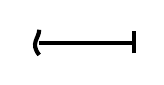
\begin{tikzpicture}[line width=1.5pt]
\draw (0,0)--(1.2,0);\draw (0,-.15)..controls (-.12,0) and (0,.06)..(0,.17);\draw (1.2,-.13)--(1.2,.16);
\end{tikzpicture}}

\figure{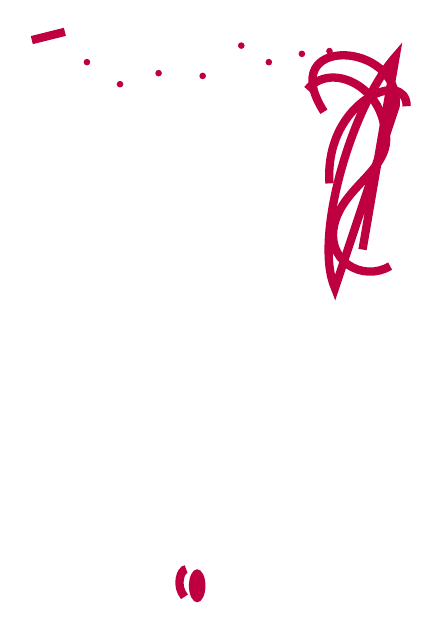
\begin{tikzpicture}[x=.7cm,y=.7cm,line width=3pt,purple]
\draw (0,4)..controls (.4,4.5) and (1.3,4.1)..(1.4,3.3)..controls (1.6,2.6) and (.7,2.3)..(.5,1.6)..controls (.3,.9) and (1,.5)..(1.5,.8);
\draw (.3,3.6)..controls (-.6,5) and (1.7,4.9)..(1.6,3.7)--(.5,.4)..controls (.1,1.3) and (.8,3.7)..(1.6,4.6)--(1,1.1);
\draw (.4,2.3)..controls (.3,3.8) and (1.8,4.4)..(1.8,3.7);
\draw (-5,4.9)--(-4.4,5.05);
\foreach \x/\y in {-4/4.5,-3.4/4.1,-2.7/4.3,-1.9/4.25,-1.2/4.8,-.7/4.5,-.1/4.65,.4/4.7} {\fill (\x,\y) circle (.06);}
\fill (-2,-5) ellipse (.15 and .3);\draw (-2.23,-5.2)..controls (-2.4,-5) and (-2.3,-4.7)..(-2.2,-4.7);
\end{tikzpicture}}
% archive foliation: 28
\scanpage{27}
\mspage{1}
$X$ surface \deleted{conforme}\inserted{hol \unsure{0}-connexe} (\unsure{pas néc cpte})

$\widetilde X$ rev. universel

\margin{\uline{NB} Ici ``surface'' sous-entend ``séparée''}

\uline{Th} Conditions équivalentes

(i) $X$ n'est pas isom. à une des trois surfaces
\[
\mathbb P^1_{\mathbb C},\ \mathbb E^1_{\mathbb C}=\mathbb P^1_{\mathbb C}\backslash\{\infty\},\quad G_{m\,\mathbb C}=\mathbb P^1_{\mathbb C}\backslash\{\infty,0\},
\]
ni à une courbe elliptique complexe

(ii) $\widetilde X$ est isomorphe à $H$ (demi-plan de Poincaré)

(iii) Toute application holomorphe $\mathbb C\longrightarrow X$ est constante

(iv) [Si $X$ est un ouvert de une droite projective complexe\deleted{]} (resp. d'une droite affine complexe)]
\[
\operatorname{card}(\deleted{\unsure{\mathbb P^1}}X'\backslash X)\ge3
\quad(\text{resp. }\operatorname{card}(\deleted{\unsure{\mathbb A^1}}X'\backslash X)\ge2).
\]

\deleted{(iv') [Si $X$ est un ouvert de \unsure{C. unif.}}

(v) [Si $X=\widehat X\backslash S$, $\widehat X$ compacte\inserted{genre $g$}, $S$ finie\inserted{card $\nu$}]
\deleted{holomorphe connexe $X'$}
\[
\unsure{2|3}g+\nu\ge3\qquad\text{i.e. }(g,\nu)\unsure{\notin|\ne}\{(0,0)(0,1)(0,2)(1,0)\}
\]
\[
\text{i.e. }\chi_c(X)<0
\]

\uline{Déf} On dit alors que $X$ est hyperbolique

\uline{Corollaire 1} Un ouvert \unsure{0}-connexe d'une surface hol. hyperbolique est hyperbolique

\uline{Corollaire 2} Soit $X$ surface hol. \uline{à bord}, \deleted{\unsure{0-co}} connexe, avec $\partial X\ne\varnothing$. Alors $\operatorname{Int}X$ est hyperbolique
% archive foliation: 29
\scanpage{28}
\mspage{2}
les surfaces suivantes :

a) le plan projectif réel ($\simeq$ Sphère conforme/antipod.) et le plan projectif réel privé d'un point (dont les rev. universels hol. resp. $\simeq\mathbb P^1_{\mathbb C}$ et $\simeq G_{m\,\mathbb C}$).

b) Les surfaces conformes associées aux courbes \deleted{elliptiques}\inserted{lisses géom. connexes} réelles $E$\inserted{de genre $1$} telles que $E(\mathbb R)=\varnothing$, en posant \deleted{$\unsure{E_{\mathbb C}}$}
\[
X=E(\mathbb C)/\text{conj. complexe}.
\]
On trouve que les $E$ en question, à isom. près, sont les $E_a^!$, $a\in\mathbb R^{*+}$\ldots

\rule{\linewidth}{0.3pt}

\uline{Question des \inserted{\unsure{la}} métriques riemanniennes}\\
\uline{canoniques sur une surface conforme}

(sans bord pour commencer)

\textcircled{1} Cas hyperbolique, Il y a une métrique canonique, à courbure constante de valeur $-1$, déduite par descente du revêtement universel $\widetilde X$.

\uline{Métrique hyperbolique}
% archive foliation: 30
\scanpage{29}
\mspage{3}
déterminée par la condition que l'aire totale de $X$ soit $=1$.

On trouve une \uline{métrique plate} caractérisée par la condition d'être invariante par translation, et d'aire \deleted{\unsure{volume}} totale égale à $1$ - donc stable par tt autom. conforme (pas seulement holomorphe). Je \unsure{sousent} que dans le cas non orienté, la métrique canonique de $X^{or}$ (qui est une courbe elliptique / $\mathbb C$) se descend à $X^{\unsure{or|an}}$.

$2'$) Cas $X\simeq\mathbb C^*$, ou\inserted{$X\simeq$} plan projectif réel privé d'un point [i.e. $X$ non orientable et $X^{or}\simeq\mathbb C^*$]. Comme dans $2$, dans le cas $X\simeq\mathbb C^*$, \deleted{plus généralement $X^{\unsure{or}}$} \deleted{\unsure{par}} descente à partir du rev. universel, on trouve une métrique canonique mod. multiplication par un scalaire $>0$, \uline{métrique plate} également.

\deleted{Comme} les autom. de $\mathbb C^*$\inserted{sont} \deleted{\unsure{précisément}}\inserted{\unsure{tt}} de la forme $z\longrightarrow az$, soit $z\longrightarrow a/z$, qui conservent la métrique [car sur $\widetilde X\simeq\mathbb C$ ils correspondent à des autom. $z\longrightarrow z+\alpha$, $z\longmapsto-z+\alpha$], Donc en \unsure{définissant|choisissant} la métrique sur $\mathbb C^*$, \deleted{\unsure{de façon}}\inserted{on}
% archive foliation: 31
\scanpage{30}
\mspage{4}
\unsure{en} la normalisant\inserted{p. ex.} de telle façon que la longueur du cercle $|z|=1$ soit \deleted{$2\pi$} $1$, on la définit sur toutes les $X\simeq\mathbb C^*$ en $=$ fait. D'ailleurs l'anti-automorphisme $z\longmapsto\bar z$ \deleted{\unsure{qui}} conserve la mesure, donc si $X\simeq\mathbb C^*$, \uline{tt} autom. conforme respecte la mesure canonique.

\margin{C'est la métrique déduite de \unsure{C! définie|celle définie} par hermitienne canonique $z\bar z$ sur $\mathbb C$, via $z\longmapsto\exp 2i\pi z$, de $\mathbb C$ sur $\mathbb C^*$.}

Il en résulte que dans le cas non orienté $X\simeq$ plan projectif réel moins $1$ pt, on peut descendre à partir de $X^{or}$ et on trouve aussi une métrique canonique plate, stable par tous les automorphismes conformes.

$2''$) Cas $X\simeq\mathbb E^1_{\mathbb C}$. Les métriques riemanniennes sur une \deleted{\unsure{courbe}} droite vectorielle complexe $L$, associées aux structures hermitiennes\inserted{déf. pos.} sur $L$, (elles sont toutes proportionnelles) ne sont pas invariantes par autom \deleted{\unsure{de}}\inserted{de} $L$, mais seulement par le sous-groupe engendré par les translations, et les \deleted{\unsure{autom.}} homothéties par des $u\in\mathbb U=\{z\in\mathbb C\mid |z|=1\}$; elles sont quasi-invariantes par autom. quelconques (lesquels sont \uline{affines}). Donc sur une $X\simeq\mathbb E^1_{\mathbb C}$, on peut définir, non \uline{une} métrique
% archive foliation: 32
\scanpage{31}
\mspage{5}
canonique stable par translations etc, mais une classe de telles mod. homothétie par $c\in\mathbb R^{*+}$ - ces métriques sont caractérisées par la condition d'être invariantes par translation [\uline{NB} $X$ a automatiquement une structure de droite affine sur $\mathbb C$]. Ces métriques \deleted{\unsure{sont définies}} ne dépendent que de la structure conforme sous-jacente.

3) \uline{Cas} \deleted{\unsure{de la sphère} $X\simeq\mathbb P^1_{\mathbb C}$} $X\simeq$ \unsure{plan} projectif réel. Dans ce \deleted{premier} \deleted{\unsure{cas}} cas, $X^{or}$ est une droite projective complexe munie d'un anti-automorphisme invol. $\sigma$ \uline{sans pt fixe} (antipodisme), ou ce qui revient au $=$, d'une métrique ``euclidienne sphérique'' compatible avec sa structure conforme. [Celle-ci, \deleted{\unsure{étant stable}}\inserted{\unsure{se normalise}} \deleted{par l'antipodisme,}\inserted{par la condition que l'aire de la surface soit $=1$}] Étant invariante par l'antipodisme, cette métrique se descend à $X$.

$3'$) Cas $X\simeq\mathbb P^1_{\mathbb C}$. Il n'y a pas de métrique riemannienne sur $X$, invariante [ou quasi-invariante] par tt automorphismes - \unsure{donc sans} structure suppl. sur $X$
% archive foliation: 33
\scanpage{32}
\mspage{6}
il n'est pas possible d'y introduire une métrique riemannienne canonique, même modulo cte. Considérons cependant la donnée d'une structure supplémentaire du type
\[
H\subset\operatorname{Aut}_{\mathrm{conf}}(X)=G
\]
où $H$ est un sous-groupe \uline{compact} de $\operatorname{Aut}_{\mathrm{conf}}(X)$ (condition \uline{nécessaire} pour que $H$, supposé fermé, invarie une métrique euclidienne sphérique comp. avec la str. conforme). Soit $H^+=H\cap\operatorname{Aut}^+(X)$ (groupe des autom. qui conservent l'orientation). OPS $X=\mathbb P(V)$, $V$ vectoriel complexe de rg $2$, \deleted{\unsure{étant}} soit $\unsure{\widetilde H|\widehat H}$ l'image inverse de $H^+$ dans $\unsure{\operatorname{SL}(V,V)|\operatorname{SL}(V)}$, c'est donc un sous-groupe cpt, qui invarie nécessairement une forme hermitienne déf. pos. sur $V$, d'où la métrique sphérique ass. sur $X$.\inserted{(normalisée par la condition $\int_X dx=1$)}, Dans le cas où \deleted{cette métrique}\inserted{la métrique} hermitienne invariante est unique mod. cte, on trouve donc une métrique\inserted{sphérique normalisée} canonique sur $X$, définie par la\inserted{seule} donnée de $H^+$. Cette métrique est $=$ invariante par $\operatorname{Norm}_G(H^+)$\deleted{\unsure{de $H$}}, et a fortiori par $H$, et à nouveau caractérisée par cette condition.
% archive foliation: 34
\scanpage{33}
\mspage{7}
Nous allons maintenant examiner de plus près le cas où \deleted{$H^+$ \unsure{invarie}} $\operatorname{Herm}^{*+}(V)^{H^+}$ n'est pas réduit à une demi-droite. On vérifie aisément que cela revient à dire que $H^+$ \deleted{\unsure{est tel}} fixe deux pts distincts $z,z'$ de $X$, donc est contenu dans le sous-groupe de $G^+$ \deleted{\unsure{défini}} formé des \unsure{pts} qui fixent $z,z'$, lequel est isom. à $\mathbb C^*$, \deleted{\unsure{et est}}\inserted{et admet un} unique sous-groupe cpt maximal \deleted{\unsure{$T$ de dim. $1$}}\inserted{$T$ isom. à $\mathbb U$.}
\deleted{Dans ce cas les métriques invariantes par}

Si $H^+\ne\{1\}$,\inserted{[alors $\{z,z'\}$ \unsure{donc|\deleted{de}} $T$ est uniquement déterminé]} les métriques invariantes par $H^+$ sont aussi celles invariantes par $T\supset H^+$,
\margin{\uline{à vérifier}}
et elles sont en corr. $1$-$1$ \deleted{\unsure{avec}} les \deleted{trajectoires}\inserted{orbites} de $T$ dans $X^*=X\setminus\{z,z'\}$, [NB $T$ opère librement sur $X^*$\deleted{\unsure{$z$}}].

La relation s'obtient en associant à tte métrique invariante par $T$, le \deleted{\unsure{point}} grand cercle ayant comme pôles $z,z'$, lequel est une \deleted{trajectoire}\inserted{orbite} sous $T$. En particulier, tte orbite\inserted{de $X^*$} sous $H^+$ (étant contenue dans une unique orbite de $T$) définit une telle métrique.

Si $H=H^+$, il n'y a \deleted{pas} rien à ajouter. Dans le
% archive foliation: 35
\scanpage{34}
\mspage{8}
cas contraire, distinguons deux cas.

a) $H^+=\{1\}$, donc $H\simeq\{1,\sigma\}$, où $\sigma$ est une anti-involution.

1) Si \deleted{\unsure{$\sigma$}} $X^\sigma=\varnothing$, $\sigma$ fixe une métrique sphérique normalisée unique, OK.

2) Si $X^\sigma\ne\varnothing$ i.e. $\sigma$ une inversion, alors le choix d'une métrique sphérique comp. avec $\sigma$ revient à celui d'une paire de pts de $X$ conjugués sous $\sigma$. En particulier, le choix d'un point\inserted{$x$} de $X$ tel que $\sigma x\ne x$ définit une telle métrique sphérique.

b) $H^+\ne\{1\}$. Considérons le\inserted{unique} tore \deleted{\unsure{$T$}} compact de dim $1$ $T$ qui contient $H^+$, et $T.H=N$, ext. de \deleted{\unsure{$\mathbb Z$}} $\mathbb Z/2\mathbb Z$ par $T$. Les éléments \deleted{\unsure{de}} $\sigma$ de $N^-$ fixent $z,z'$, ou les intervertissent, suivant que l'élément $-1$ de $N/T$ opère trivialement sur $T$, ou par symétrie $t\longmapsto t^{-1}$.
\margin{\uline{C'est l'inverse!}}
Dans le premier cas l'ext. $N$ de\inserted{$\gamma=$} $\mathbb Z/2\mathbb Z$ par $T$ est triviale
\[
\left(H^2(\gamma,T)\simeq T^\sigma/N_\sigma(T)=T/T^2\simeq0\right)
\]
dans le deuxième cas on trouve
\[
H^2(\gamma,T)\simeq T^\sigma/N_\sigma(T)\simeq\underbrace{{}_2T}_{\mathbb Z/2\mathbb Z}/0\simeq\mathbb Z/2\mathbb Z.
\]

1) $N$ ext. \uline{centrale} de \deleted{\unsure{$\mathbb Z$}}\inserted{$\gamma$} par $T$, donc $N\simeq T\times\underset{\substack{\Vert\\\{1,\sigma\}}}{\gamma}$ (\unsure{p. direct}) engendré par $T$ et une $\sigma$ \deleted{qui}\inserted{anti-involution} qui \deleted{fixe $z,z'$} intervertit $z,z'$. \deleted{On voit que} \deleted{\unsure{géodésique}}\inserted{\unsure{inversion}} celle-ci est une inversion, \deleted{\unsure{qui}}

\figure{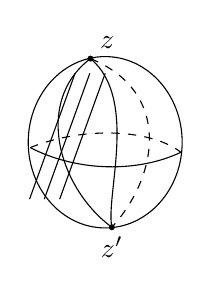
\begin{tikzpicture}[x=.85cm,y=.85cm]
\draw (0,0) ellipse (1.15 and 1.28);
\draw (-.22,1.25) .. controls (-1.08,.6) and (-.68,-.7) .. (.1,-1.27);
\draw (-.22,1.25) .. controls (.5,.65) and (.0,-.8) .. (.1,-1.27);
\draw[dashed] (-.22,1.25) .. controls (1,.75) and (.8,-.5) .. (.1,-1.27);
\draw (-1.12,-.08) .. controls (-.4,-.45) and (.5,-.45) .. (1.13,-.15);
\draw[dashed] (-1.12,-.08) .. controls (-.3,.25) and (.7,.19) .. (1.13,-.15);
\foreach \x in {-.95,-.73,-.5}{\draw (\x-.18,-.85)--(\x+.5,1.03);}
\fill (-.22,1.25) circle (.045) node[above right] {$z$};
\fill (.1,-1.27) circle (.045) node[below] {$z'$};
\end{tikzpicture}}
% archive foliation: 36
\scanpage{35}
\mspage{9}
définit donc (avec la paire $\{z,z'\}$) une métrique sphérique, ce qui sera OK. On fera attention\inserted{a priori}, que $\sigma$ n'est pas unique, il y a une ambiguïté d'ordre $2$, on peut le remplacer par $\sigma'=\varepsilon.\sigma$, où $\varepsilon$ est l'élément d'ordre $2$ de $T$. On trouve en fait que $\{\sigma,\sigma'\}$ est formé d'une inversion et d'un antipodisme.

\uline{Dém.} OPS $X=$ sphère de Riemann, $\{z,z'\}=\{\infty,0\}$, alors
\[
T=\{z\longmapsto az\mid a\in\mathbb U\text{ i.e. }a\in\mathbb C,\ |a|=1\text{ i.e. }a\bar a=1\}
\]
les \deleted{\unsure{anti}} autom. conformes anti-hol. de $\mathbb C^*$ sont
\diagram{\begin{array}{lll}
z\longmapsto a\bar z &(a\in\mathbb C^*)&\text{ceux qui fixent }0,\infty\\
z\longmapsto b/\bar z &(b\in\mathbb C^*)&\longrightarrow\ \text{intervertissent }0,\infty
\end{array}}
On voit tout de suite que ce sont les \uline{\unsure{seconds|seuls}} qui commutent à $T$. \deleted{Une telle} Si
\[
\sigma(z)=b/\bar z,\quad\text{on a}\quad\sigma^2(z)=b/\bar b\ z,
\]
donc $\sigma$ involutif ssi $b/\bar b=1$ i.e. $b\in\mathbb R^*$. Les pts fixes de $\sigma$ sont donnés par
\[
z\bar z=b
\]
\deleted{\unsure{les}} donc $\sigma$ est une inversion resp. un antipodisme, suivant que \deleted{$b\in\mathbb R$} $b>0$ ou $b<0$. Si $\sigma(z)=b/\bar z$, on a $\sigma'(z)=-b/\bar z$, \deleted{\unsure{donc}} donc si \deleted{\unsure{l'inv.}}\inserted{$\sigma$} est une inversion, $\sigma'$ est un antipodisme, et vice versa. OPS les notations choisies de telle façon que $b>0$, i.e. $\sigma$ inversion, donc $\sigma$ définit une métrique sphérique ayant \unsure{le|leur} grand cercle défini par
\[
\unsure{C|E}=\{z\in\mathbb C\mid z\bar z=b\}.
\]
% archive foliation: 37
\scanpage{36}
\mspage{10}
avec les pôles $0,\infty$. D'autre part, l'antipodisme $\sigma'z=-b/\bar z$ \deleted{\unsure{transpose}}\inserted{intervertit} $0$ et $\infty$, et \deleted{\unsure{point $z\in C$}}\inserted{transforme $C$ en lui} $=$ car $z\in C$ i.e. $z\bar z=b$ implique $\sigma'z\in C$ i.e.
\[
\underbrace{\underbrace{(\sigma'z)}_{(-b/\bar z)}\underbrace{\overline{(\sigma'z)}}_{(-b/z)}}_{b^2/z\bar z}=b
\]
Ainsi, $\sigma'$ et $(\sigma,\{0,\infty\})$ définissent la $=$ structure riemannienne sphérique. On est content!

2) $N$ est ext. \uline{non centrale} de $\gamma$ par $T$.

Cela signifie que si $\sigma\in N\setminus T$, on a
\[
\sigma.z=a\bar z,\quad\deleted{\unsure{a}}\quad(a\in\mathbb C^*).
\]
\deleted{\unsure{Donc}} on conclut
\[
\sigma^2z=a(\bar a z)=a\bar a z
\]
et la condition $\sigma^2\in T$ signifie $a\bar a=1$ d'où $a\in\mathbb U$. qui implique aussi \deleted{$\sigma^2=1$}
\[
\sigma^2=1.\qquad\text{i.e. l'extension }N\text{ est \uline{scindée}}
\]
Le produit $u_\theta\sigma$ $(\theta\in\mathbb U)$ est
\[
u_\theta\sigma(z)=(\theta a)\bar z
\]
de la $=$ forme.

Soit $\alpha$\inserted{$\in\mathbb U$} tel que
\[
a=\alpha^{\unsure{2|\sim}}=\alpha/\bar\alpha\qquad\text{donc}
\]
\[
z\in\mathbb C^\sigma\Longleftrightarrow z=\alpha\frac{\bar z}{\unsure{\bar z|\bar\alpha}}\Longleftrightarrow z/\alpha=\overline{(z/\alpha)}\quad\text{i.e.}\quad z\in\alpha\mathbb R
\]

\margin{Ici $N$ est déterminé en termes de $T$, i.e. en termes de $\{z,z'\}$, comme $T\cup N^-$, où $N^-$ est formé de \uline{toutes} les anti-involutions de $X$ qui fixent $\{z,z'\}$. Donc il n'est pas question, dans cette sorte de \unsure{données}, d'extraire une métrique riem. sphérique.}
% archive foliation: 38
\scanpage{37}
\mspage{11}
En résumé et sauf erreur

\uline{Prop.} Soit $X$ une sphère conforme \deleted{\unsure{orientée}}, $H\subset\operatorname{Aut}_{\mathrm{conf}}(X)\overset{\mathrm{def}}=G$ un sous-groupe \uline{compact} \deleted{de}, Alors

a) Il existe une métrique riemannienne sphérique normalisée sur $X$ comp. avec sa structure conforme

b) Celle-ci est unique ssi \deleted{il n'existe pas de}\inserted{$X^H=\varnothing$}

\deleted{\unsure{d}} c) Supposons \deleted{\unsure{$X^H$}} $X^H\ne\varnothing$, $H\ne\{1\}$. Alors On a \deleted{\unsure{$X$}}\inserted{ou bien} $\operatorname{card}X^H=2$, ou bien $H=\{1,\sigma\}$ où $\sigma$ est une inversion.

1) Si $\operatorname{card}X^H=2$, \deleted{Soit} $H$\inserted{$^+=H\cap G^+$. On a $X^H=X^{H^+}$, et $H^+$} est contenu dans un unique tore compact $T$, et \deleted{\unsure{les métriques}}\inserted{les métriques} sphériques riemanniennes normalisées comp., invariantes par \deleted{\unsure{$T$}} $H$, sont en corr. biunivoque avec les orbites de\inserted{$T$ dans} $(X\setminus X^H$\deleted{$)/T$} [donc tte orbite de \deleted{\unsure{$T$}} $H^+$ dans $X\setminus X^H$ définit une telle métrique]

\deleted{\unsure{b}} 2) Si $H=\{1,\sigma\}$, $\sigma$ une inversion, les métriques invariantes sous $H$ sont en corr. biunivoque avec les éléments de
\[
(X\setminus X^H)/H=(X\setminus X^\sigma)/\sigma
\]

\margin{\uline{à \unsure{rectifier|vérifier}} (\uline{NB} Il faudrait arriver à traduire en termes d'alg. linéaire, l'action d'un autom. $\unsure{u|h}\in G$ sur une métrique sphérique\unsure{.})}
% archive foliation: 39
\scanpage{38}
\mspage{12}
\uline{Récapitulation}

Soit \deleted{\unsure{toute}}\inserted{$X$} surface conforme (sans bord), \deleted{\unsure{on peut pas}}\inserted{On peut} définir sur $X$ une métrique riemannienne canonique $Q_X$,\inserted{compatible avec str. conforme} sauf dans les deux cas suivants:

a) $X\simeq\mathbb C$\inserted{(i.e. $X$ droite affine sur un corps\inserted{top} $C$ isom. à $\mathbb C$)}, alors on peut définir quand même une classe de métriques riemanniennes compatibles, mod. multiplication par un scalaire. Ce sont les métriques stables par translation, qui sont aussi quasi-inv. par tt autom. conforme de $X$. Elles sont \uline{plates} (donc à courbure nulle).

b) $X\simeq\mathbb P^1_{\mathbb C}$ (i.e. $X$ droite projective sur un corps top $C$ isom. à $\mathbb C$, ou encore $X$ sphère conforme). Alors il n'existe pas de métriques riemanniennes sur $X$ quasi-invariantes sous $G=\operatorname{Aut}X$, ni $=$ sous $\operatorname{Aut}^+(X)$.

\deleted{\unsure{Donc}} Il y a pourtant sur $X$ un \deleted{\unsure{tore}}\inserted{ens} $R(X)$ des métriques riemanniennes (dites ``sphériques normalisées'') avec $\int_X dx=1$, qui forment une orbite sous $G$. Si $H\subset G$ est un sous-groupe, il existe une $Q\in R(X)$ stable par $H$ ssi $H$ est rel. cpt; et $Q$ est unique ssi $X^H=\varnothing$. [Dans le cas $X^H\ne\varnothing$, cf proposition précédente qui détermine $R(X)^H$ dans tous les cas.]

\margin{\uline{NB} $R(X)$ est un espace \unsure{homogène} de dim $3$}
% archive foliation: 40
\scanpage{39}
\mspage{13}
% archive foliation: 41
[NB \deleted{\unsure{On}} pense notamment au cas où $X$ est associé à une \uline{carte}, et $H$ est le groupe des autom. de cette carte, qui est fini --- la condition $X^H=\varnothing$ signifie aussi qu'il n'y a pas de facette de la carte fixe par $H$.]

Dans tous les cas où $Q_X$ est définie, $Q_X$ est hyperbolique (i.e. : courbure $<0$) ssi $X$ est hyperbolique, et alors $Q_X$ est de courbure \inserted{constante} égale à $-1$. D'autre part $Q_X$ est \uline{plate} \deleted{dans les cas} (ou encore, de courbure nulle) ssi $\widetilde X\simeq\mathbb C$ [y inclus le cas a) ci-dessus, où on a encore une $Q_X$ mod cte]. Le cas restant est celui du plan projectif réel, conforme, \deleted{qui est} \deleted{dans} lequel $Q_X$ est une métrique homogène, de courbure cte \deleted{égale à} et $>0$.

Donc chaque fois que $Q_X$ est définie, ou définie mod cte, il est à courbure constante, \deleted{et c'est} Il en est encore de $=$ des $Q_{X,H}$ quand $X\simeq\mathbb P^1_{\mathbb C}$ et $H\subset\mathrm{Aut}_{\mathrm{conf}}X$ est cpt et tq que $X^H=\varnothing$, on trouve une métrique sph. euclidienne, donc de courbure constante $>0$.

\margin{\uline{NB} Pour tte $X$ 0-connexe conforme on \deleted{\unsure{a}} a dans l'ensemble \deleted{des \unsure{métriques}} $\mathrm{Riem}(X)$ des métr. riemanniennes comp. avec la str. conforme une orbite canonique sous $\mathrm{Aut}_{\mathrm{conf}}(X)$, qui est réduite à 1 pt dans tous les cas, sauf les cas a) et b) de la p. 12, où dans le cas a), on trouve une demi-droite dans $\mathrm{Riem}(X)$, et dans le cas b), une variété de dim 3 (\deleted{\unsure{qui}}\inserted{telles} \deleted{\unsure{que}} que $Q,Q'\in R(X)$, $Q\ne Q'$ implique $Q'$ et $Q$ \uline{non} prop). Notion des métriques riemanniennes distinguées (a un sens aussi dans le cas \unsure{disconnexe}).}
\scanpage{40}
\mspage{14}
% archive foliation: 42
\uline{Cas des surfaces conformes à bord} (pas néc. cptes)

On utilise l'équivalence de catégories
\diagram{\begin{array}{c@{\quad\simeq\quad}l}
\text{surfaces conformes à bord}&\text{surfaces holomorphes sans bord,}\\
&\text{munies d'une anti-involution.}
\end{array}}
\diagram{\begin{tikzcd}[column sep=large,row sep=large]
X \arrow[r,mapsto] & (X'=X^{or},\sigma)\\
X=X'/\sigma & (X',\sigma) \arrow[l,mapsto]
\end{tikzcd}}

On dit que $X$ est hyperbolique ssi $X^{or}$ est hyperbolique \inserted{(i.e. ses comp. connexes les 2 ou 1)}. Quand $X$ est sans bord, on a $\widetilde X\simeq\widetilde{X^{or}}$ (car $X^{or}$ est un rev. étale de $X$) donc $X$ est hyperbolique au sens des réflexions précédentes, ssi il l'est en ce nouveau sens.

Si $X$ est compact, \inserted{donc $X^{or}$ aussi,} comme on a
\[
\chi(X^{or})=2\chi(X),
\]
et que $\chi(X^{or})<0\Longleftrightarrow X^{or}$ hyperbolique, on trouve
\[
X\text{ hyperbolique}\Longleftrightarrow\chi(X)<0.
\]
P.ex. si $X$ est holomorphe 0-connexe, de type $g,\nu$, cela signifie que
\[
2g\unsure{+|-}2+\nu\geq1\qquad\text{i.e}\quad2g+\nu\geq3.
\]
Mais on se gardera de confondre cette condition avec celle que $\mathrm{Int}\,X$ soit hyperbolique, ce qui est tjrs vrai sauf si $\nu=0$, $g\in\{0,1\}$\ldots
\scanpage{41}
\mspage{15}
% archive foliation: 43
Si $X$ est une surface conforme hyperbolique, alors la métrique canonique hyperbolique sur $X^{or}$ se descend en une métrique hyperbolique sur $X$, pour laquelle le bord est géodésique.

Plus généralement, chaque fois que $X^{or}$ est muni d'une métrique canonique, invariante par autom. conformes [ou seulement par anti-involutions, ce qui est le cas aussi si $X^{or}\simeq\mathbb C$] alors celle-ci se descend à $X$, avec bord géodésique.

Quand $X$ est sans bord, \deleted{\unsure{alors si elle}} alors \deleted{\unsure{si}} la métrique obtenue sur $X$ est celle déjà envisagée --- \deleted{\unsure{elle}} \inserted{il y en a} dans tous les cas, sauf $X\simeq\mathbb P^1_{\mathbb C}$. On fera attention cependant que lorsque $X$ est le plan projectif réel, la deuxième prescription sans plus ne fournit \uline{pas} de métrique --- elle le fait si on exige que la métrique sur $X^{or}$ soit en $R(X^{or})$, \uline{et} stable par $\sigma$ (ce qui la détermine sans ambiguïté). \deleted{De $=$} \inserted{\deleted{Dans le} En sens inverse}, dans le cas $X\simeq\mathbb C$, $X^{or}\simeq\mathbb C\amalg\mathbb C$, le procédé direct donne une classe des métriques (mod cte), la deuxième
\scanpage{42}
\mspage{16}
% archive foliation: 44
ne donne quelque chose que si on la complète par la prescription que l'on prend une métrique ``distinguée'' sur $X^{or}$ qui soit stable par $\sigma$.

Considérons maintenant les seuls cas nouveaux --- ceux où $X$ est 0-connexe et $\partial X\ne\varnothing$, correspondant à un $X^{or}=\mathcal X$ connexe, munie d'une anti-involution $\sigma$ telle que $\mathcal X^\sigma\ne\varnothing$. Les seuls cas problématiques pour l'existence d'une métrique canonique sur $X$, sont les suivants :

a') $\mathcal X\simeq\mathbb C$. \deleted{Les \unsure{anti.}} \inserted{OPS} $\mathcal X=\mathbb C$. Les anti-aut. de $\mathbb C$ sont
\[
z\longmapsto a\overline z+b\qquad(a\in\mathbb C^*,\ b\in\mathbb C).
\]
Si on prend une anti-involution à pts fixes, OPS que 0 est pt fixe, donc $b=0$; donc \deleted{l'application est $z\longmapsto a\overline z$}
\[
\sigma z=a\overline z\qquad\text{avec }a\overline a=1\quad\text{i.e }|a|=1\quad\text{i.e }a\in\mathbb U
\]
(pour avoir $\sigma^2=\mathrm{id}$) soit
\deleted{l'ens des pts fixes est}
\[
\sigma z=\alpha^2\overline z=\frac\alpha{\overline\alpha}\overline z\qquad\text{si }a=\alpha^2,\quad\alpha\in\mathbb U,
\]
et l'ens des pts fixes est
\[
\mathbb C^\sigma=\alpha.\mathbb R.
\]
\margin{symétrie p.r. à la droite $\alpha.\mathbb R$}
\scanpage{43}
\mspage{17}
% archive foliation: 45
En fait, les anti-involutions de $\mathbb C$ ont toutes des pts fixes, et ce sont les symétries orth. p.r. à des droites réelles (pas néc. passant par l'origine) dans $\mathbb C$. La surface à bord conforme correspondante est isom. à un \uuline{demi-plan} (avec bord). On note que tte métrique \inserted{sur $\mathcal X$,} quasi-invariante par autom. conformes, est invariante par autom. d'ordre fini, en particulier par $\sigma$. Donc il y a sur $X$ une classe \inserted{can.} de métriques riemanniennes, mod. cte.

\uline{NB} \deleted{\unsure{Le}} Le modèle de $X$ envisagé est le demi-plan supérieur \deleted{$\unsure{\mathbb C}$}
\[
\overline{\mathbb H}=\{z\in\mathbb C\mid\mathrm{Im}\,z\geq0\}.
\]
Le groupe des autom. de $\overline H$, isom. au groupe des autom. de la droite affine $\mathbb C$ qui commutent à $\sigma:z\longmapsto\overline z$, est \uline{le groupe affine réel}
\scanpage{44}
\mspage{18}
% archive foliation: 46
b') Cas $\mathcal X\simeq\mathbb P^1_{\mathbb C}$, $\sigma$ une inversion --- laquelle définit une structure de droite projective réelle --- on trouve \deleted{le disque} pour $X$ un \uline{disque}. Pour obtenir une métrique distinguée sur $\mathcal X$ invariante par $\sigma$, il faut se donner un pt du disque ouvert $X\setminus\partial X$

\figure{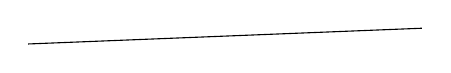
\begin{tikzpicture}\draw (0,0)--(5,.2);\end{tikzpicture}}

En résumé, tte surface conforme à bord 0-connexe admet une unique métrique Riemannienne distinguée, sauf dans les quatre cas suivants

a) a') Cas $X\simeq\mathbb C$, ou $X\simeq\unsure{\overline{\mathbb H}|\mathbb H}=\{z\in\mathbb C\mid\mathrm{Im}\,z\geq0\}$ [droite affine complexe, demi-plan à bord défini par une droite affine réelle], on a alors une classe de métriques mod constante, qui forment une orbite sous $\mathrm{Aut}\,X$.

b) b') $X\simeq\mathbb P^1_{\mathbb C}$ ou $X\simeq\text{disque}$ [droite projective complexe ou \deleted{\unsure{demidisque fermé}} défini par droite projective réelle] --- il y a alors un ens. de métriques distinguées dépendant de 3 paramètres réels resp. de 2 paramètres réels, également orbite sous $\mathrm{Aut}\,X$.
\scanpage{45}
\mspage{\unsure{1'|19}}
% archive foliation: 47
\uline{Corollaire 3} Soit $\underset{\text{ouvert}\atop\text{0-connexe}}{X}\subset X'$, $X'$ hol. 0-connexe. Alors $X$ est hyperbolique, sauf dans les cas suivants :

a) $X'$ est $\simeq\mathbb P^1_{\mathbb C}$ (resp. $\mathbb E^1_{\mathbb C}$, resp. $\mathbb G_{m\mathbb C}$), et $\operatorname{card}(X\setminus X')\leq2$ (resp. $\leq1$, resp. $=0$)

b) $X'$ est compacte de genre 1 et $X=X'$.

\uline{Remarque} Soit \deleted{\unsure{e}} $X$ une surface conforme 0-connexe (pas néc. orientable). On dit encore que $X$ est hyperbolique si $\widetilde X\simeq\mathbb H$, ou ce qui revient au $=$, si tte application conforme $\mathbb C\longrightarrow X$ est constante.

\margin{ou encore si le rev. \deleted{\unsure{absolu}} \inserted{des} orientations (qui est une surf. holomorphe) est hyperbolique.}

Ainsi les surfaces conformes \inserted{ss. bord,} 0-connexes \uline{non} hyperboliques sont, en plus des quatre cas énumérés dans (i) ci-dessus, les quotients de telles surfaces par des anti-involutions sans pts fixes. On trouve donc de plus
\scanpage{46}
\mspage{\unsure{2'|21}}
% archive foliation: 48
Dans le cas où $X$ est compact, on trouve que c'est la seule métrique riemannienne (comp. avec la structure conforme) qui soit de courbure constante égale à $-1$.

2) Cas \deleted{elliptique} comp. et (orientables ou non) de genre 1. Dans le cas orienté, i.e. celui d'une courbe elliptique complexe, dont le rev. universel est une droite complexe, on a sur celui-ci une métrique canonique mod scalaire (métrique hermitienne) invariante par translations (et quasi-inv. par tout autom. i.e. par transformation affine), qu'on peut descendre à $X$. La constante multiplicative est
\scanpage{48}
\mspage{1}
% archive foliation: 50
\unsure{10369CNU|10369GNU}\qquad 15.1.

$X$ \deleted{non singulière} \inserted{lisse de type $g,\nu$} (sur $\overline{\mathbb Q}$)

$Y$ stable non lisse type $(g,\nu)$ avec propagateur normal $N$ d'où un groupe fondamental \unsure{ét.}\deleted{\unsure{indép.}} $\unsure{\Pi|\pi}_1([Y,N])$

\diagram{\begin{array}{c}X\overset f{\underset T\simeq}Y\end{array}} un isomorphisme de Teichmüller.

\uline{NB} Cet isomorphisme induit un isom de groupes extérieurs \deleted{\unsure{celui est de}} (\unsure{il est déterminé} plus bas)
\diagram{\begin{tikzcd}[column sep=large]\unsure{\Pi|\pi}_1(X)\arrow[r]&\unsure{\Pi|\pi}_1([Y,N])\end{tikzcd}}

Quand on se donne un ``pt base sur $X$'' (ordinaire ou à l'infini), et un sur $[Y,N]$ (alors --- et de plus distinct des pts singuliers de $Y$) on a une notion d'isom de Teichmüller respectant les pts marqués, \deleted{et \unsure{d'un}} (on suppose qu'ils sont tous deux à distance finie, ou tous deux à l'infini). Et on trouve alors un isom de groupes (pas ext. !)
\diagram{\begin{tikzcd}[column sep=large]\unsure{\Pi|\pi}_1(X,\unsure{\bullet|x})\arrow[r]&\unsure{\Pi|\pi}_1([Y,N],y)\end{tikzcd}}

En tout état de cause, \deleted{\unsure{les}} l'isom extérieur déjà n'est pas compatible avec les actions ext. de $\operatorname{Gal}(\overline{\mathbb Q}/K)$, $K$ \inserted{\unsure{est}} une extension finie de $\overline{\mathbb Q}/\mathbb Q$ assez grande

\margin{\uline{NB} Mettre en évidence \uline{trois} classes de conjugaison d'\deleted{éléments} hom. $\widehat{\mathbb Z}(1)\longrightarrow\unsure{\Pi|\pi}_1(X)$ (deux seulement si $\nu=0$, l'une des trois est alors ``le vide'').}
\scanpage{49}
\mspage{2}
% archive foliation: 51
\deleted{\texttt{/*JOB=CRAY2,ACCT=\unsure{*********|********},ALL=M06,MSGL=N}\\
\texttt{// JOB MSGLEVEL=(1,1),MSGCLASS=A}\\
\texttt{// EXEC PGM=IEFBR14}}

\uline{À examiner} : a) Extension de la conjecture fondamentale en géom. alg. anabélienne aux courbes anabéliennes \deleted{\unsure{stables}} singulières (stables, avec propagateur normal). \unsure{?|P}

b) Pour une $Y$, \figure{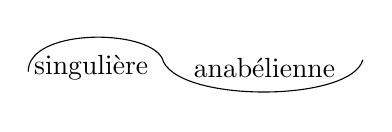
\begin{tikzpicture}[baseline=(a.base)]
\node[inner sep=1pt] (a) at (0,0) {singulière};
\node[inner sep=1pt] (b) at (2.2,0) {anabélienne};
\draw (-.8,-.05)..controls(-.8,.5)and(.7,.5)..(.9,.12)..controls(1.05,-.45)and(3.3,-.45)..(3.45,.1);
\end{tikzpicture}} donnée (sur corps $K$ de t.f. sur $\mathbb Q$), est-il vrai qu'on récupère les \unsure{él.|cl.} de \deleted{\unsure{pts}} $\operatorname{Sing}(Y)\cup\underbrace{\text{Pts marqués}}_{Y_\infty}$ en termes des \inserted{classes de conj.} sous-groupes de $\unsure{\Pi|\pi}_1(Y)$ isom. à $\widehat{\mathbb Z}$, et ext. invariants par $\unsure{\Pi|\pi}_1(K)$ (l'opération de $\unsure{\Pi|\pi}_1(K)$ dessus se fait automatiquement via le caractère cyclotomique)

c) S'inspirant des compactifications MD des $M_{g\nu}$, définir ce que c'est qu'une compactification anabélienne d'une variété lisse anabélienne (sur un corps $\inserted{K}$ de car. 0, qu'on peut supposer être de type fini sur $\mathbb Q$). Comportement par spécialisation ???
\scanpage{50}
% archive foliation: 52
Générateurs et relations pour les groupoïdes et groupes de Teichmüller (spéciaux et ordinaires, évt. toriques\ldots)

Je m'attends à trouver trois types de présentations à propriétés complémentaires --- mais toutes à signification arithmétique :

a) Présentation par ``\uline{pantalons}'' ou ``\uline{triades}''. Elle revient à travailler sur les pts à l'infini ``les plus \unsure{cubiques|critiques}'' sur les multiplicités modulaires, et semble (d'après l'exemple de $\mathcal T_{0,4}^{+!}$) commode surtout pour exprimer des groupes du type $T_{g,\nu}^{+!}$ (ou $T_{g;I}^{+}$).

b) Présentation par ``boîte'' complète de pièces de Légo (\unsure{voire|voir} des boîtes encore plus complètes) à l'aide des \inserted{\uline{groupes d'}}\uline{automorphismes} \inserted{\uline{\unsure{stricts}}} de ces pièces, et certains ``chemins'' de déformation particuliers allant de certaines pièces à d'autres. Exemples frappants : $T_{0,4}^+$ (\unsure{connu!|connus!}), ou
\[
T_{1,1}^+\simeq\mathrm{SL}(2,\mathbb Z)\quad\text{engendré par }\rho,\sigma\quad\text{avec }\rho^{\unsure{3}}=\sigma^2,
\]
\[
\rho^6\ (=\sigma^4)=1.
\]

c) Présentations \uline{par involutions}, qui sont dans $\mathcal T_{g\nu}^{-}$. Exemple typique $\unsure{\mathbb T|T}_{11}\simeq\mathrm{GL}(2,\mathbb Z)$ \deleted{\unsure{eng}} (\deleted{\unsure{Origine}} aux Groupes cartographiques triangulés) engendré par trois réflexions $r_1,r_2,r_3$ avec
\[
(r_1r_2)^2=(r_2r_3)^3,\quad(r_1r_2)^4\bigl(=(r_2r_3)^6\bigr)=1.
\]
\scanpage{51}
% archive foliation: 53
% Printed matter is upright in the supplied scan; the manuscript is inverted.
\texttt{//*\quad CRAY2\quad 0369\qquad I}
\figure{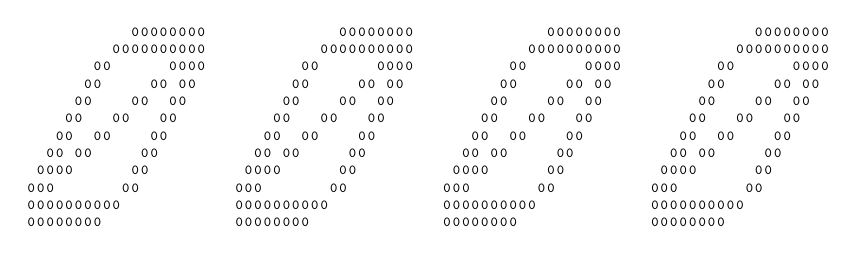
\begin{tikzpicture}[x=0.12cm,y=0.22cm]
\node[inner sep=0pt,font=\ttfamily\tiny] at (11,0){0};
\node[inner sep=0pt,font=\ttfamily\tiny] at (12,0){0};
\node[inner sep=0pt,font=\ttfamily\tiny] at (13,0){0};
\node[inner sep=0pt,font=\ttfamily\tiny] at (14,0){0};
\node[inner sep=0pt,font=\ttfamily\tiny] at (15,0){0};
\node[inner sep=0pt,font=\ttfamily\tiny] at (16,0){0};
\node[inner sep=0pt,font=\ttfamily\tiny] at (17,0){0};
\node[inner sep=0pt,font=\ttfamily\tiny] at (18,0){0};
\node[inner sep=0pt,font=\ttfamily\tiny] at (33,0){0};
\node[inner sep=0pt,font=\ttfamily\tiny] at (34,0){0};
\node[inner sep=0pt,font=\ttfamily\tiny] at (35,0){0};
\node[inner sep=0pt,font=\ttfamily\tiny] at (36,0){0};
\node[inner sep=0pt,font=\ttfamily\tiny] at (37,0){0};
\node[inner sep=0pt,font=\ttfamily\tiny] at (38,0){0};
\node[inner sep=0pt,font=\ttfamily\tiny] at (39,0){0};
\node[inner sep=0pt,font=\ttfamily\tiny] at (40,0){0};
\node[inner sep=0pt,font=\ttfamily\tiny] at (55,0){0};
\node[inner sep=0pt,font=\ttfamily\tiny] at (56,0){0};
\node[inner sep=0pt,font=\ttfamily\tiny] at (57,0){0};
\node[inner sep=0pt,font=\ttfamily\tiny] at (58,0){0};
\node[inner sep=0pt,font=\ttfamily\tiny] at (59,0){0};
\node[inner sep=0pt,font=\ttfamily\tiny] at (60,0){0};
\node[inner sep=0pt,font=\ttfamily\tiny] at (61,0){0};
\node[inner sep=0pt,font=\ttfamily\tiny] at (62,0){0};
\node[inner sep=0pt,font=\ttfamily\tiny] at (77,0){0};
\node[inner sep=0pt,font=\ttfamily\tiny] at (78,0){0};
\node[inner sep=0pt,font=\ttfamily\tiny] at (79,0){0};
\node[inner sep=0pt,font=\ttfamily\tiny] at (80,0){0};
\node[inner sep=0pt,font=\ttfamily\tiny] at (81,0){0};
\node[inner sep=0pt,font=\ttfamily\tiny] at (82,0){0};
\node[inner sep=0pt,font=\ttfamily\tiny] at (83,0){0};
\node[inner sep=0pt,font=\ttfamily\tiny] at (84,0){0};
\node[inner sep=0pt,font=\ttfamily\tiny] at (9,-1){0};
\node[inner sep=0pt,font=\ttfamily\tiny] at (10,-1){0};
\node[inner sep=0pt,font=\ttfamily\tiny] at (11,-1){0};
\node[inner sep=0pt,font=\ttfamily\tiny] at (12,-1){0};
\node[inner sep=0pt,font=\ttfamily\tiny] at (13,-1){0};
\node[inner sep=0pt,font=\ttfamily\tiny] at (14,-1){0};
\node[inner sep=0pt,font=\ttfamily\tiny] at (15,-1){0};
\node[inner sep=0pt,font=\ttfamily\tiny] at (16,-1){0};
\node[inner sep=0pt,font=\ttfamily\tiny] at (17,-1){0};
\node[inner sep=0pt,font=\ttfamily\tiny] at (18,-1){0};
\node[inner sep=0pt,font=\ttfamily\tiny] at (31,-1){0};
\node[inner sep=0pt,font=\ttfamily\tiny] at (32,-1){0};
\node[inner sep=0pt,font=\ttfamily\tiny] at (33,-1){0};
\node[inner sep=0pt,font=\ttfamily\tiny] at (34,-1){0};
\node[inner sep=0pt,font=\ttfamily\tiny] at (35,-1){0};
\node[inner sep=0pt,font=\ttfamily\tiny] at (36,-1){0};
\node[inner sep=0pt,font=\ttfamily\tiny] at (37,-1){0};
\node[inner sep=0pt,font=\ttfamily\tiny] at (38,-1){0};
\node[inner sep=0pt,font=\ttfamily\tiny] at (39,-1){0};
\node[inner sep=0pt,font=\ttfamily\tiny] at (40,-1){0};
\node[inner sep=0pt,font=\ttfamily\tiny] at (53,-1){0};
\node[inner sep=0pt,font=\ttfamily\tiny] at (54,-1){0};
\node[inner sep=0pt,font=\ttfamily\tiny] at (55,-1){0};
\node[inner sep=0pt,font=\ttfamily\tiny] at (56,-1){0};
\node[inner sep=0pt,font=\ttfamily\tiny] at (57,-1){0};
\node[inner sep=0pt,font=\ttfamily\tiny] at (58,-1){0};
\node[inner sep=0pt,font=\ttfamily\tiny] at (59,-1){0};
\node[inner sep=0pt,font=\ttfamily\tiny] at (60,-1){0};
\node[inner sep=0pt,font=\ttfamily\tiny] at (61,-1){0};
\node[inner sep=0pt,font=\ttfamily\tiny] at (62,-1){0};
\node[inner sep=0pt,font=\ttfamily\tiny] at (75,-1){0};
\node[inner sep=0pt,font=\ttfamily\tiny] at (76,-1){0};
\node[inner sep=0pt,font=\ttfamily\tiny] at (77,-1){0};
\node[inner sep=0pt,font=\ttfamily\tiny] at (78,-1){0};
\node[inner sep=0pt,font=\ttfamily\tiny] at (79,-1){0};
\node[inner sep=0pt,font=\ttfamily\tiny] at (80,-1){0};
\node[inner sep=0pt,font=\ttfamily\tiny] at (81,-1){0};
\node[inner sep=0pt,font=\ttfamily\tiny] at (82,-1){0};
\node[inner sep=0pt,font=\ttfamily\tiny] at (83,-1){0};
\node[inner sep=0pt,font=\ttfamily\tiny] at (84,-1){0};
\node[inner sep=0pt,font=\ttfamily\tiny] at (7,-2){0};
\node[inner sep=0pt,font=\ttfamily\tiny] at (8,-2){0};
\node[inner sep=0pt,font=\ttfamily\tiny] at (15,-2){0};
\node[inner sep=0pt,font=\ttfamily\tiny] at (16,-2){0};
\node[inner sep=0pt,font=\ttfamily\tiny] at (17,-2){0};
\node[inner sep=0pt,font=\ttfamily\tiny] at (18,-2){0};
\node[inner sep=0pt,font=\ttfamily\tiny] at (29,-2){0};
\node[inner sep=0pt,font=\ttfamily\tiny] at (30,-2){0};
\node[inner sep=0pt,font=\ttfamily\tiny] at (37,-2){0};
\node[inner sep=0pt,font=\ttfamily\tiny] at (38,-2){0};
\node[inner sep=0pt,font=\ttfamily\tiny] at (39,-2){0};
\node[inner sep=0pt,font=\ttfamily\tiny] at (40,-2){0};
\node[inner sep=0pt,font=\ttfamily\tiny] at (51,-2){0};
\node[inner sep=0pt,font=\ttfamily\tiny] at (52,-2){0};
\node[inner sep=0pt,font=\ttfamily\tiny] at (59,-2){0};
\node[inner sep=0pt,font=\ttfamily\tiny] at (60,-2){0};
\node[inner sep=0pt,font=\ttfamily\tiny] at (61,-2){0};
\node[inner sep=0pt,font=\ttfamily\tiny] at (62,-2){0};
\node[inner sep=0pt,font=\ttfamily\tiny] at (73,-2){0};
\node[inner sep=0pt,font=\ttfamily\tiny] at (74,-2){0};
\node[inner sep=0pt,font=\ttfamily\tiny] at (81,-2){0};
\node[inner sep=0pt,font=\ttfamily\tiny] at (82,-2){0};
\node[inner sep=0pt,font=\ttfamily\tiny] at (83,-2){0};
\node[inner sep=0pt,font=\ttfamily\tiny] at (84,-2){0};
\node[inner sep=0pt,font=\ttfamily\tiny] at (6,-3){0};
\node[inner sep=0pt,font=\ttfamily\tiny] at (7,-3){0};
\node[inner sep=0pt,font=\ttfamily\tiny] at (13,-3){0};
\node[inner sep=0pt,font=\ttfamily\tiny] at (14,-3){0};
\node[inner sep=0pt,font=\ttfamily\tiny] at (16,-3){0};
\node[inner sep=0pt,font=\ttfamily\tiny] at (17,-3){0};
\node[inner sep=0pt,font=\ttfamily\tiny] at (28,-3){0};
\node[inner sep=0pt,font=\ttfamily\tiny] at (29,-3){0};
\node[inner sep=0pt,font=\ttfamily\tiny] at (35,-3){0};
\node[inner sep=0pt,font=\ttfamily\tiny] at (36,-3){0};
\node[inner sep=0pt,font=\ttfamily\tiny] at (38,-3){0};
\node[inner sep=0pt,font=\ttfamily\tiny] at (39,-3){0};
\node[inner sep=0pt,font=\ttfamily\tiny] at (50,-3){0};
\node[inner sep=0pt,font=\ttfamily\tiny] at (51,-3){0};
\node[inner sep=0pt,font=\ttfamily\tiny] at (57,-3){0};
\node[inner sep=0pt,font=\ttfamily\tiny] at (58,-3){0};
\node[inner sep=0pt,font=\ttfamily\tiny] at (60,-3){0};
\node[inner sep=0pt,font=\ttfamily\tiny] at (61,-3){0};
\node[inner sep=0pt,font=\ttfamily\tiny] at (72,-3){0};
\node[inner sep=0pt,font=\ttfamily\tiny] at (73,-3){0};
\node[inner sep=0pt,font=\ttfamily\tiny] at (79,-3){0};
\node[inner sep=0pt,font=\ttfamily\tiny] at (80,-3){0};
\node[inner sep=0pt,font=\ttfamily\tiny] at (82,-3){0};
\node[inner sep=0pt,font=\ttfamily\tiny] at (83,-3){0};
\node[inner sep=0pt,font=\ttfamily\tiny] at (5,-4){0};
\node[inner sep=0pt,font=\ttfamily\tiny] at (6,-4){0};
\node[inner sep=0pt,font=\ttfamily\tiny] at (11,-4){0};
\node[inner sep=0pt,font=\ttfamily\tiny] at (12,-4){0};
\node[inner sep=0pt,font=\ttfamily\tiny] at (15,-4){0};
\node[inner sep=0pt,font=\ttfamily\tiny] at (16,-4){0};
\node[inner sep=0pt,font=\ttfamily\tiny] at (27,-4){0};
\node[inner sep=0pt,font=\ttfamily\tiny] at (28,-4){0};
\node[inner sep=0pt,font=\ttfamily\tiny] at (33,-4){0};
\node[inner sep=0pt,font=\ttfamily\tiny] at (34,-4){0};
\node[inner sep=0pt,font=\ttfamily\tiny] at (37,-4){0};
\node[inner sep=0pt,font=\ttfamily\tiny] at (38,-4){0};
\node[inner sep=0pt,font=\ttfamily\tiny] at (49,-4){0};
\node[inner sep=0pt,font=\ttfamily\tiny] at (50,-4){0};
\node[inner sep=0pt,font=\ttfamily\tiny] at (55,-4){0};
\node[inner sep=0pt,font=\ttfamily\tiny] at (56,-4){0};
\node[inner sep=0pt,font=\ttfamily\tiny] at (59,-4){0};
\node[inner sep=0pt,font=\ttfamily\tiny] at (60,-4){0};
\node[inner sep=0pt,font=\ttfamily\tiny] at (71,-4){0};
\node[inner sep=0pt,font=\ttfamily\tiny] at (72,-4){0};
\node[inner sep=0pt,font=\ttfamily\tiny] at (77,-4){0};
\node[inner sep=0pt,font=\ttfamily\tiny] at (78,-4){0};
\node[inner sep=0pt,font=\ttfamily\tiny] at (81,-4){0};
\node[inner sep=0pt,font=\ttfamily\tiny] at (82,-4){0};
\node[inner sep=0pt,font=\ttfamily\tiny] at (4,-5){0};
\node[inner sep=0pt,font=\ttfamily\tiny] at (5,-5){0};
\node[inner sep=0pt,font=\ttfamily\tiny] at (9,-5){0};
\node[inner sep=0pt,font=\ttfamily\tiny] at (10,-5){0};
\node[inner sep=0pt,font=\ttfamily\tiny] at (14,-5){0};
\node[inner sep=0pt,font=\ttfamily\tiny] at (15,-5){0};
\node[inner sep=0pt,font=\ttfamily\tiny] at (26,-5){0};
\node[inner sep=0pt,font=\ttfamily\tiny] at (27,-5){0};
\node[inner sep=0pt,font=\ttfamily\tiny] at (31,-5){0};
\node[inner sep=0pt,font=\ttfamily\tiny] at (32,-5){0};
\node[inner sep=0pt,font=\ttfamily\tiny] at (36,-5){0};
\node[inner sep=0pt,font=\ttfamily\tiny] at (37,-5){0};
\node[inner sep=0pt,font=\ttfamily\tiny] at (48,-5){0};
\node[inner sep=0pt,font=\ttfamily\tiny] at (49,-5){0};
\node[inner sep=0pt,font=\ttfamily\tiny] at (53,-5){0};
\node[inner sep=0pt,font=\ttfamily\tiny] at (54,-5){0};
\node[inner sep=0pt,font=\ttfamily\tiny] at (58,-5){0};
\node[inner sep=0pt,font=\ttfamily\tiny] at (59,-5){0};
\node[inner sep=0pt,font=\ttfamily\tiny] at (70,-5){0};
\node[inner sep=0pt,font=\ttfamily\tiny] at (71,-5){0};
\node[inner sep=0pt,font=\ttfamily\tiny] at (75,-5){0};
\node[inner sep=0pt,font=\ttfamily\tiny] at (76,-5){0};
\node[inner sep=0pt,font=\ttfamily\tiny] at (80,-5){0};
\node[inner sep=0pt,font=\ttfamily\tiny] at (81,-5){0};
\node[inner sep=0pt,font=\ttfamily\tiny] at (3,-6){0};
\node[inner sep=0pt,font=\ttfamily\tiny] at (4,-6){0};
\node[inner sep=0pt,font=\ttfamily\tiny] at (7,-6){0};
\node[inner sep=0pt,font=\ttfamily\tiny] at (8,-6){0};
\node[inner sep=0pt,font=\ttfamily\tiny] at (13,-6){0};
\node[inner sep=0pt,font=\ttfamily\tiny] at (14,-6){0};
\node[inner sep=0pt,font=\ttfamily\tiny] at (25,-6){0};
\node[inner sep=0pt,font=\ttfamily\tiny] at (26,-6){0};
\node[inner sep=0pt,font=\ttfamily\tiny] at (29,-6){0};
\node[inner sep=0pt,font=\ttfamily\tiny] at (30,-6){0};
\node[inner sep=0pt,font=\ttfamily\tiny] at (35,-6){0};
\node[inner sep=0pt,font=\ttfamily\tiny] at (36,-6){0};
\node[inner sep=0pt,font=\ttfamily\tiny] at (47,-6){0};
\node[inner sep=0pt,font=\ttfamily\tiny] at (48,-6){0};
\node[inner sep=0pt,font=\ttfamily\tiny] at (51,-6){0};
\node[inner sep=0pt,font=\ttfamily\tiny] at (52,-6){0};
\node[inner sep=0pt,font=\ttfamily\tiny] at (57,-6){0};
\node[inner sep=0pt,font=\ttfamily\tiny] at (58,-6){0};
\node[inner sep=0pt,font=\ttfamily\tiny] at (69,-6){0};
\node[inner sep=0pt,font=\ttfamily\tiny] at (70,-6){0};
\node[inner sep=0pt,font=\ttfamily\tiny] at (73,-6){0};
\node[inner sep=0pt,font=\ttfamily\tiny] at (74,-6){0};
\node[inner sep=0pt,font=\ttfamily\tiny] at (79,-6){0};
\node[inner sep=0pt,font=\ttfamily\tiny] at (80,-6){0};
\node[inner sep=0pt,font=\ttfamily\tiny] at (2,-7){0};
\node[inner sep=0pt,font=\ttfamily\tiny] at (3,-7){0};
\node[inner sep=0pt,font=\ttfamily\tiny] at (5,-7){0};
\node[inner sep=0pt,font=\ttfamily\tiny] at (6,-7){0};
\node[inner sep=0pt,font=\ttfamily\tiny] at (12,-7){0};
\node[inner sep=0pt,font=\ttfamily\tiny] at (13,-7){0};
\node[inner sep=0pt,font=\ttfamily\tiny] at (24,-7){0};
\node[inner sep=0pt,font=\ttfamily\tiny] at (25,-7){0};
\node[inner sep=0pt,font=\ttfamily\tiny] at (27,-7){0};
\node[inner sep=0pt,font=\ttfamily\tiny] at (28,-7){0};
\node[inner sep=0pt,font=\ttfamily\tiny] at (34,-7){0};
\node[inner sep=0pt,font=\ttfamily\tiny] at (35,-7){0};
\node[inner sep=0pt,font=\ttfamily\tiny] at (46,-7){0};
\node[inner sep=0pt,font=\ttfamily\tiny] at (47,-7){0};
\node[inner sep=0pt,font=\ttfamily\tiny] at (49,-7){0};
\node[inner sep=0pt,font=\ttfamily\tiny] at (50,-7){0};
\node[inner sep=0pt,font=\ttfamily\tiny] at (56,-7){0};
\node[inner sep=0pt,font=\ttfamily\tiny] at (57,-7){0};
\node[inner sep=0pt,font=\ttfamily\tiny] at (68,-7){0};
\node[inner sep=0pt,font=\ttfamily\tiny] at (69,-7){0};
\node[inner sep=0pt,font=\ttfamily\tiny] at (71,-7){0};
\node[inner sep=0pt,font=\ttfamily\tiny] at (72,-7){0};
\node[inner sep=0pt,font=\ttfamily\tiny] at (78,-7){0};
\node[inner sep=0pt,font=\ttfamily\tiny] at (79,-7){0};
\node[inner sep=0pt,font=\ttfamily\tiny] at (1,-8){0};
\node[inner sep=0pt,font=\ttfamily\tiny] at (2,-8){0};
\node[inner sep=0pt,font=\ttfamily\tiny] at (3,-8){0};
\node[inner sep=0pt,font=\ttfamily\tiny] at (4,-8){0};
\node[inner sep=0pt,font=\ttfamily\tiny] at (11,-8){0};
\node[inner sep=0pt,font=\ttfamily\tiny] at (12,-8){0};
\node[inner sep=0pt,font=\ttfamily\tiny] at (23,-8){0};
\node[inner sep=0pt,font=\ttfamily\tiny] at (24,-8){0};
\node[inner sep=0pt,font=\ttfamily\tiny] at (25,-8){0};
\node[inner sep=0pt,font=\ttfamily\tiny] at (26,-8){0};
\node[inner sep=0pt,font=\ttfamily\tiny] at (33,-8){0};
\node[inner sep=0pt,font=\ttfamily\tiny] at (34,-8){0};
\node[inner sep=0pt,font=\ttfamily\tiny] at (45,-8){0};
\node[inner sep=0pt,font=\ttfamily\tiny] at (46,-8){0};
\node[inner sep=0pt,font=\ttfamily\tiny] at (47,-8){0};
\node[inner sep=0pt,font=\ttfamily\tiny] at (48,-8){0};
\node[inner sep=0pt,font=\ttfamily\tiny] at (55,-8){0};
\node[inner sep=0pt,font=\ttfamily\tiny] at (56,-8){0};
\node[inner sep=0pt,font=\ttfamily\tiny] at (67,-8){0};
\node[inner sep=0pt,font=\ttfamily\tiny] at (68,-8){0};
\node[inner sep=0pt,font=\ttfamily\tiny] at (69,-8){0};
\node[inner sep=0pt,font=\ttfamily\tiny] at (70,-8){0};
\node[inner sep=0pt,font=\ttfamily\tiny] at (77,-8){0};
\node[inner sep=0pt,font=\ttfamily\tiny] at (78,-8){0};
\node[inner sep=0pt,font=\ttfamily\tiny] at (0,-9){0};
\node[inner sep=0pt,font=\ttfamily\tiny] at (1,-9){0};
\node[inner sep=0pt,font=\ttfamily\tiny] at (2,-9){0};
\node[inner sep=0pt,font=\ttfamily\tiny] at (10,-9){0};
\node[inner sep=0pt,font=\ttfamily\tiny] at (11,-9){0};
\node[inner sep=0pt,font=\ttfamily\tiny] at (22,-9){0};
\node[inner sep=0pt,font=\ttfamily\tiny] at (23,-9){0};
\node[inner sep=0pt,font=\ttfamily\tiny] at (24,-9){0};
\node[inner sep=0pt,font=\ttfamily\tiny] at (32,-9){0};
\node[inner sep=0pt,font=\ttfamily\tiny] at (33,-9){0};
\node[inner sep=0pt,font=\ttfamily\tiny] at (44,-9){0};
\node[inner sep=0pt,font=\ttfamily\tiny] at (45,-9){0};
\node[inner sep=0pt,font=\ttfamily\tiny] at (46,-9){0};
\node[inner sep=0pt,font=\ttfamily\tiny] at (54,-9){0};
\node[inner sep=0pt,font=\ttfamily\tiny] at (55,-9){0};
\node[inner sep=0pt,font=\ttfamily\tiny] at (66,-9){0};
\node[inner sep=0pt,font=\ttfamily\tiny] at (67,-9){0};
\node[inner sep=0pt,font=\ttfamily\tiny] at (68,-9){0};
\node[inner sep=0pt,font=\ttfamily\tiny] at (76,-9){0};
\node[inner sep=0pt,font=\ttfamily\tiny] at (77,-9){0};
\node[inner sep=0pt,font=\ttfamily\tiny] at (0,-10){0};
\node[inner sep=0pt,font=\ttfamily\tiny] at (1,-10){0};
\node[inner sep=0pt,font=\ttfamily\tiny] at (2,-10){0};
\node[inner sep=0pt,font=\ttfamily\tiny] at (3,-10){0};
\node[inner sep=0pt,font=\ttfamily\tiny] at (4,-10){0};
\node[inner sep=0pt,font=\ttfamily\tiny] at (5,-10){0};
\node[inner sep=0pt,font=\ttfamily\tiny] at (6,-10){0};
\node[inner sep=0pt,font=\ttfamily\tiny] at (7,-10){0};
\node[inner sep=0pt,font=\ttfamily\tiny] at (8,-10){0};
\node[inner sep=0pt,font=\ttfamily\tiny] at (9,-10){0};
\node[inner sep=0pt,font=\ttfamily\tiny] at (22,-10){0};
\node[inner sep=0pt,font=\ttfamily\tiny] at (23,-10){0};
\node[inner sep=0pt,font=\ttfamily\tiny] at (24,-10){0};
\node[inner sep=0pt,font=\ttfamily\tiny] at (25,-10){0};
\node[inner sep=0pt,font=\ttfamily\tiny] at (26,-10){0};
\node[inner sep=0pt,font=\ttfamily\tiny] at (27,-10){0};
\node[inner sep=0pt,font=\ttfamily\tiny] at (28,-10){0};
\node[inner sep=0pt,font=\ttfamily\tiny] at (29,-10){0};
\node[inner sep=0pt,font=\ttfamily\tiny] at (30,-10){0};
\node[inner sep=0pt,font=\ttfamily\tiny] at (31,-10){0};
\node[inner sep=0pt,font=\ttfamily\tiny] at (44,-10){0};
\node[inner sep=0pt,font=\ttfamily\tiny] at (45,-10){0};
\node[inner sep=0pt,font=\ttfamily\tiny] at (46,-10){0};
\node[inner sep=0pt,font=\ttfamily\tiny] at (47,-10){0};
\node[inner sep=0pt,font=\ttfamily\tiny] at (48,-10){0};
\node[inner sep=0pt,font=\ttfamily\tiny] at (49,-10){0};
\node[inner sep=0pt,font=\ttfamily\tiny] at (50,-10){0};
\node[inner sep=0pt,font=\ttfamily\tiny] at (51,-10){0};
\node[inner sep=0pt,font=\ttfamily\tiny] at (52,-10){0};
\node[inner sep=0pt,font=\ttfamily\tiny] at (53,-10){0};
\node[inner sep=0pt,font=\ttfamily\tiny] at (66,-10){0};
\node[inner sep=0pt,font=\ttfamily\tiny] at (67,-10){0};
\node[inner sep=0pt,font=\ttfamily\tiny] at (68,-10){0};
\node[inner sep=0pt,font=\ttfamily\tiny] at (69,-10){0};
\node[inner sep=0pt,font=\ttfamily\tiny] at (70,-10){0};
\node[inner sep=0pt,font=\ttfamily\tiny] at (71,-10){0};
\node[inner sep=0pt,font=\ttfamily\tiny] at (72,-10){0};
\node[inner sep=0pt,font=\ttfamily\tiny] at (73,-10){0};
\node[inner sep=0pt,font=\ttfamily\tiny] at (74,-10){0};
\node[inner sep=0pt,font=\ttfamily\tiny] at (75,-10){0};
\node[inner sep=0pt,font=\ttfamily\tiny] at (0,-11){0};
\node[inner sep=0pt,font=\ttfamily\tiny] at (1,-11){0};
\node[inner sep=0pt,font=\ttfamily\tiny] at (2,-11){0};
\node[inner sep=0pt,font=\ttfamily\tiny] at (3,-11){0};
\node[inner sep=0pt,font=\ttfamily\tiny] at (4,-11){0};
\node[inner sep=0pt,font=\ttfamily\tiny] at (5,-11){0};
\node[inner sep=0pt,font=\ttfamily\tiny] at (6,-11){0};
\node[inner sep=0pt,font=\ttfamily\tiny] at (7,-11){0};
\node[inner sep=0pt,font=\ttfamily\tiny] at (22,-11){0};
\node[inner sep=0pt,font=\ttfamily\tiny] at (23,-11){0};
\node[inner sep=0pt,font=\ttfamily\tiny] at (24,-11){0};
\node[inner sep=0pt,font=\ttfamily\tiny] at (25,-11){0};
\node[inner sep=0pt,font=\ttfamily\tiny] at (26,-11){0};
\node[inner sep=0pt,font=\ttfamily\tiny] at (27,-11){0};
\node[inner sep=0pt,font=\ttfamily\tiny] at (28,-11){0};
\node[inner sep=0pt,font=\ttfamily\tiny] at (29,-11){0};
\node[inner sep=0pt,font=\ttfamily\tiny] at (44,-11){0};
\node[inner sep=0pt,font=\ttfamily\tiny] at (45,-11){0};
\node[inner sep=0pt,font=\ttfamily\tiny] at (46,-11){0};
\node[inner sep=0pt,font=\ttfamily\tiny] at (47,-11){0};
\node[inner sep=0pt,font=\ttfamily\tiny] at (48,-11){0};
\node[inner sep=0pt,font=\ttfamily\tiny] at (49,-11){0};
\node[inner sep=0pt,font=\ttfamily\tiny] at (50,-11){0};
\node[inner sep=0pt,font=\ttfamily\tiny] at (51,-11){0};
\node[inner sep=0pt,font=\ttfamily\tiny] at (66,-11){0};
\node[inner sep=0pt,font=\ttfamily\tiny] at (67,-11){0};
\node[inner sep=0pt,font=\ttfamily\tiny] at (68,-11){0};
\node[inner sep=0pt,font=\ttfamily\tiny] at (69,-11){0};
\node[inner sep=0pt,font=\ttfamily\tiny] at (70,-11){0};
\node[inner sep=0pt,font=\ttfamily\tiny] at (71,-11){0};
\node[inner sep=0pt,font=\ttfamily\tiny] at (72,-11){0};
\node[inner sep=0pt,font=\ttfamily\tiny] at (73,-11){0};
\end{tikzpicture}}

\figure{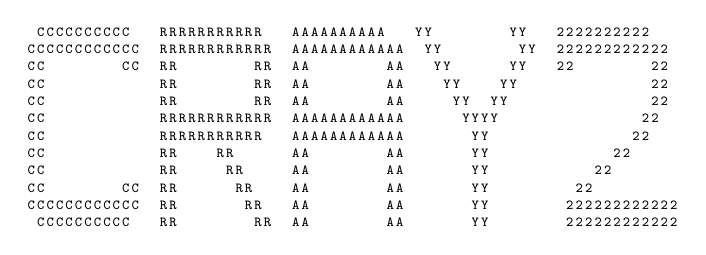
\begin{tikzpicture}[x=0.12cm,y=0.22cm]
\node[inner sep=0pt,font=\ttfamily\tiny] at (1,0){C};
\node[inner sep=0pt,font=\ttfamily\tiny] at (2,0){C};
\node[inner sep=0pt,font=\ttfamily\tiny] at (3,0){C};
\node[inner sep=0pt,font=\ttfamily\tiny] at (4,0){C};
\node[inner sep=0pt,font=\ttfamily\tiny] at (5,0){C};
\node[inner sep=0pt,font=\ttfamily\tiny] at (6,0){C};
\node[inner sep=0pt,font=\ttfamily\tiny] at (7,0){C};
\node[inner sep=0pt,font=\ttfamily\tiny] at (8,0){C};
\node[inner sep=0pt,font=\ttfamily\tiny] at (9,0){C};
\node[inner sep=0pt,font=\ttfamily\tiny] at (10,0){C};
\node[inner sep=0pt,font=\ttfamily\tiny] at (14,0){R};
\node[inner sep=0pt,font=\ttfamily\tiny] at (15,0){R};
\node[inner sep=0pt,font=\ttfamily\tiny] at (16,0){R};
\node[inner sep=0pt,font=\ttfamily\tiny] at (17,0){R};
\node[inner sep=0pt,font=\ttfamily\tiny] at (18,0){R};
\node[inner sep=0pt,font=\ttfamily\tiny] at (19,0){R};
\node[inner sep=0pt,font=\ttfamily\tiny] at (20,0){R};
\node[inner sep=0pt,font=\ttfamily\tiny] at (21,0){R};
\node[inner sep=0pt,font=\ttfamily\tiny] at (22,0){R};
\node[inner sep=0pt,font=\ttfamily\tiny] at (23,0){R};
\node[inner sep=0pt,font=\ttfamily\tiny] at (24,0){R};
\node[inner sep=0pt,font=\ttfamily\tiny] at (28,0){A};
\node[inner sep=0pt,font=\ttfamily\tiny] at (29,0){A};
\node[inner sep=0pt,font=\ttfamily\tiny] at (30,0){A};
\node[inner sep=0pt,font=\ttfamily\tiny] at (31,0){A};
\node[inner sep=0pt,font=\ttfamily\tiny] at (32,0){A};
\node[inner sep=0pt,font=\ttfamily\tiny] at (33,0){A};
\node[inner sep=0pt,font=\ttfamily\tiny] at (34,0){A};
\node[inner sep=0pt,font=\ttfamily\tiny] at (35,0){A};
\node[inner sep=0pt,font=\ttfamily\tiny] at (36,0){A};
\node[inner sep=0pt,font=\ttfamily\tiny] at (37,0){A};
\node[inner sep=0pt,font=\ttfamily\tiny] at (41,0){Y};
\node[inner sep=0pt,font=\ttfamily\tiny] at (42,0){Y};
\node[inner sep=0pt,font=\ttfamily\tiny] at (51,0){Y};
\node[inner sep=0pt,font=\ttfamily\tiny] at (52,0){Y};
\node[inner sep=0pt,font=\ttfamily\tiny] at (56,0){2};
\node[inner sep=0pt,font=\ttfamily\tiny] at (57,0){2};
\node[inner sep=0pt,font=\ttfamily\tiny] at (58,0){2};
\node[inner sep=0pt,font=\ttfamily\tiny] at (59,0){2};
\node[inner sep=0pt,font=\ttfamily\tiny] at (60,0){2};
\node[inner sep=0pt,font=\ttfamily\tiny] at (61,0){2};
\node[inner sep=0pt,font=\ttfamily\tiny] at (62,0){2};
\node[inner sep=0pt,font=\ttfamily\tiny] at (63,0){2};
\node[inner sep=0pt,font=\ttfamily\tiny] at (64,0){2};
\node[inner sep=0pt,font=\ttfamily\tiny] at (65,0){2};
\node[inner sep=0pt,font=\ttfamily\tiny] at (0,-1){C};
\node[inner sep=0pt,font=\ttfamily\tiny] at (1,-1){C};
\node[inner sep=0pt,font=\ttfamily\tiny] at (2,-1){C};
\node[inner sep=0pt,font=\ttfamily\tiny] at (3,-1){C};
\node[inner sep=0pt,font=\ttfamily\tiny] at (4,-1){C};
\node[inner sep=0pt,font=\ttfamily\tiny] at (5,-1){C};
\node[inner sep=0pt,font=\ttfamily\tiny] at (6,-1){C};
\node[inner sep=0pt,font=\ttfamily\tiny] at (7,-1){C};
\node[inner sep=0pt,font=\ttfamily\tiny] at (8,-1){C};
\node[inner sep=0pt,font=\ttfamily\tiny] at (9,-1){C};
\node[inner sep=0pt,font=\ttfamily\tiny] at (10,-1){C};
\node[inner sep=0pt,font=\ttfamily\tiny] at (11,-1){C};
\node[inner sep=0pt,font=\ttfamily\tiny] at (14,-1){R};
\node[inner sep=0pt,font=\ttfamily\tiny] at (15,-1){R};
\node[inner sep=0pt,font=\ttfamily\tiny] at (16,-1){R};
\node[inner sep=0pt,font=\ttfamily\tiny] at (17,-1){R};
\node[inner sep=0pt,font=\ttfamily\tiny] at (18,-1){R};
\node[inner sep=0pt,font=\ttfamily\tiny] at (19,-1){R};
\node[inner sep=0pt,font=\ttfamily\tiny] at (20,-1){R};
\node[inner sep=0pt,font=\ttfamily\tiny] at (21,-1){R};
\node[inner sep=0pt,font=\ttfamily\tiny] at (22,-1){R};
\node[inner sep=0pt,font=\ttfamily\tiny] at (23,-1){R};
\node[inner sep=0pt,font=\ttfamily\tiny] at (24,-1){R};
\node[inner sep=0pt,font=\ttfamily\tiny] at (25,-1){R};
\node[inner sep=0pt,font=\ttfamily\tiny] at (28,-1){A};
\node[inner sep=0pt,font=\ttfamily\tiny] at (29,-1){A};
\node[inner sep=0pt,font=\ttfamily\tiny] at (30,-1){A};
\node[inner sep=0pt,font=\ttfamily\tiny] at (31,-1){A};
\node[inner sep=0pt,font=\ttfamily\tiny] at (32,-1){A};
\node[inner sep=0pt,font=\ttfamily\tiny] at (33,-1){A};
\node[inner sep=0pt,font=\ttfamily\tiny] at (34,-1){A};
\node[inner sep=0pt,font=\ttfamily\tiny] at (35,-1){A};
\node[inner sep=0pt,font=\ttfamily\tiny] at (36,-1){A};
\node[inner sep=0pt,font=\ttfamily\tiny] at (37,-1){A};
\node[inner sep=0pt,font=\ttfamily\tiny] at (38,-1){A};
\node[inner sep=0pt,font=\ttfamily\tiny] at (39,-1){A};
\node[inner sep=0pt,font=\ttfamily\tiny] at (42,-1){Y};
\node[inner sep=0pt,font=\ttfamily\tiny] at (43,-1){Y};
\node[inner sep=0pt,font=\ttfamily\tiny] at (52,-1){Y};
\node[inner sep=0pt,font=\ttfamily\tiny] at (53,-1){Y};
\node[inner sep=0pt,font=\ttfamily\tiny] at (56,-1){2};
\node[inner sep=0pt,font=\ttfamily\tiny] at (57,-1){2};
\node[inner sep=0pt,font=\ttfamily\tiny] at (58,-1){2};
\node[inner sep=0pt,font=\ttfamily\tiny] at (59,-1){2};
\node[inner sep=0pt,font=\ttfamily\tiny] at (60,-1){2};
\node[inner sep=0pt,font=\ttfamily\tiny] at (61,-1){2};
\node[inner sep=0pt,font=\ttfamily\tiny] at (62,-1){2};
\node[inner sep=0pt,font=\ttfamily\tiny] at (63,-1){2};
\node[inner sep=0pt,font=\ttfamily\tiny] at (64,-1){2};
\node[inner sep=0pt,font=\ttfamily\tiny] at (65,-1){2};
\node[inner sep=0pt,font=\ttfamily\tiny] at (66,-1){2};
\node[inner sep=0pt,font=\ttfamily\tiny] at (67,-1){2};
\node[inner sep=0pt,font=\ttfamily\tiny] at (0,-2){C};
\node[inner sep=0pt,font=\ttfamily\tiny] at (1,-2){C};
\node[inner sep=0pt,font=\ttfamily\tiny] at (10,-2){C};
\node[inner sep=0pt,font=\ttfamily\tiny] at (11,-2){C};
\node[inner sep=0pt,font=\ttfamily\tiny] at (14,-2){R};
\node[inner sep=0pt,font=\ttfamily\tiny] at (15,-2){R};
\node[inner sep=0pt,font=\ttfamily\tiny] at (24,-2){R};
\node[inner sep=0pt,font=\ttfamily\tiny] at (25,-2){R};
\node[inner sep=0pt,font=\ttfamily\tiny] at (28,-2){A};
\node[inner sep=0pt,font=\ttfamily\tiny] at (29,-2){A};
\node[inner sep=0pt,font=\ttfamily\tiny] at (38,-2){A};
\node[inner sep=0pt,font=\ttfamily\tiny] at (39,-2){A};
\node[inner sep=0pt,font=\ttfamily\tiny] at (43,-2){Y};
\node[inner sep=0pt,font=\ttfamily\tiny] at (44,-2){Y};
\node[inner sep=0pt,font=\ttfamily\tiny] at (51,-2){Y};
\node[inner sep=0pt,font=\ttfamily\tiny] at (52,-2){Y};
\node[inner sep=0pt,font=\ttfamily\tiny] at (56,-2){2};
\node[inner sep=0pt,font=\ttfamily\tiny] at (57,-2){2};
\node[inner sep=0pt,font=\ttfamily\tiny] at (66,-2){2};
\node[inner sep=0pt,font=\ttfamily\tiny] at (67,-2){2};
\node[inner sep=0pt,font=\ttfamily\tiny] at (0,-3){C};
\node[inner sep=0pt,font=\ttfamily\tiny] at (1,-3){C};
\node[inner sep=0pt,font=\ttfamily\tiny] at (14,-3){R};
\node[inner sep=0pt,font=\ttfamily\tiny] at (15,-3){R};
\node[inner sep=0pt,font=\ttfamily\tiny] at (24,-3){R};
\node[inner sep=0pt,font=\ttfamily\tiny] at (25,-3){R};
\node[inner sep=0pt,font=\ttfamily\tiny] at (28,-3){A};
\node[inner sep=0pt,font=\ttfamily\tiny] at (29,-3){A};
\node[inner sep=0pt,font=\ttfamily\tiny] at (38,-3){A};
\node[inner sep=0pt,font=\ttfamily\tiny] at (39,-3){A};
\node[inner sep=0pt,font=\ttfamily\tiny] at (44,-3){Y};
\node[inner sep=0pt,font=\ttfamily\tiny] at (45,-3){Y};
\node[inner sep=0pt,font=\ttfamily\tiny] at (50,-3){Y};
\node[inner sep=0pt,font=\ttfamily\tiny] at (51,-3){Y};
\node[inner sep=0pt,font=\ttfamily\tiny] at (66,-3){2};
\node[inner sep=0pt,font=\ttfamily\tiny] at (67,-3){2};
\node[inner sep=0pt,font=\ttfamily\tiny] at (0,-4){C};
\node[inner sep=0pt,font=\ttfamily\tiny] at (1,-4){C};
\node[inner sep=0pt,font=\ttfamily\tiny] at (14,-4){R};
\node[inner sep=0pt,font=\ttfamily\tiny] at (15,-4){R};
\node[inner sep=0pt,font=\ttfamily\tiny] at (24,-4){R};
\node[inner sep=0pt,font=\ttfamily\tiny] at (25,-4){R};
\node[inner sep=0pt,font=\ttfamily\tiny] at (28,-4){A};
\node[inner sep=0pt,font=\ttfamily\tiny] at (29,-4){A};
\node[inner sep=0pt,font=\ttfamily\tiny] at (38,-4){A};
\node[inner sep=0pt,font=\ttfamily\tiny] at (39,-4){A};
\node[inner sep=0pt,font=\ttfamily\tiny] at (45,-4){Y};
\node[inner sep=0pt,font=\ttfamily\tiny] at (46,-4){Y};
\node[inner sep=0pt,font=\ttfamily\tiny] at (49,-4){Y};
\node[inner sep=0pt,font=\ttfamily\tiny] at (50,-4){Y};
\node[inner sep=0pt,font=\ttfamily\tiny] at (66,-4){2};
\node[inner sep=0pt,font=\ttfamily\tiny] at (67,-4){2};
\node[inner sep=0pt,font=\ttfamily\tiny] at (0,-5){C};
\node[inner sep=0pt,font=\ttfamily\tiny] at (1,-5){C};
\node[inner sep=0pt,font=\ttfamily\tiny] at (14,-5){R};
\node[inner sep=0pt,font=\ttfamily\tiny] at (15,-5){R};
\node[inner sep=0pt,font=\ttfamily\tiny] at (16,-5){R};
\node[inner sep=0pt,font=\ttfamily\tiny] at (17,-5){R};
\node[inner sep=0pt,font=\ttfamily\tiny] at (18,-5){R};
\node[inner sep=0pt,font=\ttfamily\tiny] at (19,-5){R};
\node[inner sep=0pt,font=\ttfamily\tiny] at (20,-5){R};
\node[inner sep=0pt,font=\ttfamily\tiny] at (21,-5){R};
\node[inner sep=0pt,font=\ttfamily\tiny] at (22,-5){R};
\node[inner sep=0pt,font=\ttfamily\tiny] at (23,-5){R};
\node[inner sep=0pt,font=\ttfamily\tiny] at (24,-5){R};
\node[inner sep=0pt,font=\ttfamily\tiny] at (25,-5){R};
\node[inner sep=0pt,font=\ttfamily\tiny] at (28,-5){A};
\node[inner sep=0pt,font=\ttfamily\tiny] at (29,-5){A};
\node[inner sep=0pt,font=\ttfamily\tiny] at (30,-5){A};
\node[inner sep=0pt,font=\ttfamily\tiny] at (31,-5){A};
\node[inner sep=0pt,font=\ttfamily\tiny] at (32,-5){A};
\node[inner sep=0pt,font=\ttfamily\tiny] at (33,-5){A};
\node[inner sep=0pt,font=\ttfamily\tiny] at (34,-5){A};
\node[inner sep=0pt,font=\ttfamily\tiny] at (35,-5){A};
\node[inner sep=0pt,font=\ttfamily\tiny] at (36,-5){A};
\node[inner sep=0pt,font=\ttfamily\tiny] at (37,-5){A};
\node[inner sep=0pt,font=\ttfamily\tiny] at (38,-5){A};
\node[inner sep=0pt,font=\ttfamily\tiny] at (39,-5){A};
\node[inner sep=0pt,font=\ttfamily\tiny] at (46,-5){Y};
\node[inner sep=0pt,font=\ttfamily\tiny] at (47,-5){Y};
\node[inner sep=0pt,font=\ttfamily\tiny] at (48,-5){Y};
\node[inner sep=0pt,font=\ttfamily\tiny] at (49,-5){Y};
\node[inner sep=0pt,font=\ttfamily\tiny] at (65,-5){2};
\node[inner sep=0pt,font=\ttfamily\tiny] at (66,-5){2};
\node[inner sep=0pt,font=\ttfamily\tiny] at (0,-6){C};
\node[inner sep=0pt,font=\ttfamily\tiny] at (1,-6){C};
\node[inner sep=0pt,font=\ttfamily\tiny] at (14,-6){R};
\node[inner sep=0pt,font=\ttfamily\tiny] at (15,-6){R};
\node[inner sep=0pt,font=\ttfamily\tiny] at (16,-6){R};
\node[inner sep=0pt,font=\ttfamily\tiny] at (17,-6){R};
\node[inner sep=0pt,font=\ttfamily\tiny] at (18,-6){R};
\node[inner sep=0pt,font=\ttfamily\tiny] at (19,-6){R};
\node[inner sep=0pt,font=\ttfamily\tiny] at (20,-6){R};
\node[inner sep=0pt,font=\ttfamily\tiny] at (21,-6){R};
\node[inner sep=0pt,font=\ttfamily\tiny] at (22,-6){R};
\node[inner sep=0pt,font=\ttfamily\tiny] at (23,-6){R};
\node[inner sep=0pt,font=\ttfamily\tiny] at (24,-6){R};
\node[inner sep=0pt,font=\ttfamily\tiny] at (28,-6){A};
\node[inner sep=0pt,font=\ttfamily\tiny] at (29,-6){A};
\node[inner sep=0pt,font=\ttfamily\tiny] at (30,-6){A};
\node[inner sep=0pt,font=\ttfamily\tiny] at (31,-6){A};
\node[inner sep=0pt,font=\ttfamily\tiny] at (32,-6){A};
\node[inner sep=0pt,font=\ttfamily\tiny] at (33,-6){A};
\node[inner sep=0pt,font=\ttfamily\tiny] at (34,-6){A};
\node[inner sep=0pt,font=\ttfamily\tiny] at (35,-6){A};
\node[inner sep=0pt,font=\ttfamily\tiny] at (36,-6){A};
\node[inner sep=0pt,font=\ttfamily\tiny] at (37,-6){A};
\node[inner sep=0pt,font=\ttfamily\tiny] at (38,-6){A};
\node[inner sep=0pt,font=\ttfamily\tiny] at (39,-6){A};
\node[inner sep=0pt,font=\ttfamily\tiny] at (47,-6){Y};
\node[inner sep=0pt,font=\ttfamily\tiny] at (48,-6){Y};
\node[inner sep=0pt,font=\ttfamily\tiny] at (64,-6){2};
\node[inner sep=0pt,font=\ttfamily\tiny] at (65,-6){2};
\node[inner sep=0pt,font=\ttfamily\tiny] at (0,-7){C};
\node[inner sep=0pt,font=\ttfamily\tiny] at (1,-7){C};
\node[inner sep=0pt,font=\ttfamily\tiny] at (14,-7){R};
\node[inner sep=0pt,font=\ttfamily\tiny] at (15,-7){R};
\node[inner sep=0pt,font=\ttfamily\tiny] at (20,-7){R};
\node[inner sep=0pt,font=\ttfamily\tiny] at (21,-7){R};
\node[inner sep=0pt,font=\ttfamily\tiny] at (28,-7){A};
\node[inner sep=0pt,font=\ttfamily\tiny] at (29,-7){A};
\node[inner sep=0pt,font=\ttfamily\tiny] at (38,-7){A};
\node[inner sep=0pt,font=\ttfamily\tiny] at (39,-7){A};
\node[inner sep=0pt,font=\ttfamily\tiny] at (47,-7){Y};
\node[inner sep=0pt,font=\ttfamily\tiny] at (48,-7){Y};
\node[inner sep=0pt,font=\ttfamily\tiny] at (62,-7){2};
\node[inner sep=0pt,font=\ttfamily\tiny] at (63,-7){2};
\node[inner sep=0pt,font=\ttfamily\tiny] at (0,-8){C};
\node[inner sep=0pt,font=\ttfamily\tiny] at (1,-8){C};
\node[inner sep=0pt,font=\ttfamily\tiny] at (14,-8){R};
\node[inner sep=0pt,font=\ttfamily\tiny] at (15,-8){R};
\node[inner sep=0pt,font=\ttfamily\tiny] at (21,-8){R};
\node[inner sep=0pt,font=\ttfamily\tiny] at (22,-8){R};
\node[inner sep=0pt,font=\ttfamily\tiny] at (28,-8){A};
\node[inner sep=0pt,font=\ttfamily\tiny] at (29,-8){A};
\node[inner sep=0pt,font=\ttfamily\tiny] at (38,-8){A};
\node[inner sep=0pt,font=\ttfamily\tiny] at (39,-8){A};
\node[inner sep=0pt,font=\ttfamily\tiny] at (47,-8){Y};
\node[inner sep=0pt,font=\ttfamily\tiny] at (48,-8){Y};
\node[inner sep=0pt,font=\ttfamily\tiny] at (60,-8){2};
\node[inner sep=0pt,font=\ttfamily\tiny] at (61,-8){2};
\node[inner sep=0pt,font=\ttfamily\tiny] at (0,-9){C};
\node[inner sep=0pt,font=\ttfamily\tiny] at (1,-9){C};
\node[inner sep=0pt,font=\ttfamily\tiny] at (10,-9){C};
\node[inner sep=0pt,font=\ttfamily\tiny] at (11,-9){C};
\node[inner sep=0pt,font=\ttfamily\tiny] at (14,-9){R};
\node[inner sep=0pt,font=\ttfamily\tiny] at (15,-9){R};
\node[inner sep=0pt,font=\ttfamily\tiny] at (22,-9){R};
\node[inner sep=0pt,font=\ttfamily\tiny] at (23,-9){R};
\node[inner sep=0pt,font=\ttfamily\tiny] at (28,-9){A};
\node[inner sep=0pt,font=\ttfamily\tiny] at (29,-9){A};
\node[inner sep=0pt,font=\ttfamily\tiny] at (38,-9){A};
\node[inner sep=0pt,font=\ttfamily\tiny] at (39,-9){A};
\node[inner sep=0pt,font=\ttfamily\tiny] at (47,-9){Y};
\node[inner sep=0pt,font=\ttfamily\tiny] at (48,-9){Y};
\node[inner sep=0pt,font=\ttfamily\tiny] at (58,-9){2};
\node[inner sep=0pt,font=\ttfamily\tiny] at (59,-9){2};
\node[inner sep=0pt,font=\ttfamily\tiny] at (0,-10){C};
\node[inner sep=0pt,font=\ttfamily\tiny] at (1,-10){C};
\node[inner sep=0pt,font=\ttfamily\tiny] at (2,-10){C};
\node[inner sep=0pt,font=\ttfamily\tiny] at (3,-10){C};
\node[inner sep=0pt,font=\ttfamily\tiny] at (4,-10){C};
\node[inner sep=0pt,font=\ttfamily\tiny] at (5,-10){C};
\node[inner sep=0pt,font=\ttfamily\tiny] at (6,-10){C};
\node[inner sep=0pt,font=\ttfamily\tiny] at (7,-10){C};
\node[inner sep=0pt,font=\ttfamily\tiny] at (8,-10){C};
\node[inner sep=0pt,font=\ttfamily\tiny] at (9,-10){C};
\node[inner sep=0pt,font=\ttfamily\tiny] at (10,-10){C};
\node[inner sep=0pt,font=\ttfamily\tiny] at (11,-10){C};
\node[inner sep=0pt,font=\ttfamily\tiny] at (14,-10){R};
\node[inner sep=0pt,font=\ttfamily\tiny] at (15,-10){R};
\node[inner sep=0pt,font=\ttfamily\tiny] at (23,-10){R};
\node[inner sep=0pt,font=\ttfamily\tiny] at (24,-10){R};
\node[inner sep=0pt,font=\ttfamily\tiny] at (28,-10){A};
\node[inner sep=0pt,font=\ttfamily\tiny] at (29,-10){A};
\node[inner sep=0pt,font=\ttfamily\tiny] at (38,-10){A};
\node[inner sep=0pt,font=\ttfamily\tiny] at (39,-10){A};
\node[inner sep=0pt,font=\ttfamily\tiny] at (47,-10){Y};
\node[inner sep=0pt,font=\ttfamily\tiny] at (48,-10){Y};
\node[inner sep=0pt,font=\ttfamily\tiny] at (57,-10){2};
\node[inner sep=0pt,font=\ttfamily\tiny] at (58,-10){2};
\node[inner sep=0pt,font=\ttfamily\tiny] at (59,-10){2};
\node[inner sep=0pt,font=\ttfamily\tiny] at (60,-10){2};
\node[inner sep=0pt,font=\ttfamily\tiny] at (61,-10){2};
\node[inner sep=0pt,font=\ttfamily\tiny] at (62,-10){2};
\node[inner sep=0pt,font=\ttfamily\tiny] at (63,-10){2};
\node[inner sep=0pt,font=\ttfamily\tiny] at (64,-10){2};
\node[inner sep=0pt,font=\ttfamily\tiny] at (65,-10){2};
\node[inner sep=0pt,font=\ttfamily\tiny] at (66,-10){2};
\node[inner sep=0pt,font=\ttfamily\tiny] at (67,-10){2};
\node[inner sep=0pt,font=\ttfamily\tiny] at (68,-10){2};
\node[inner sep=0pt,font=\ttfamily\tiny] at (1,-11){C};
\node[inner sep=0pt,font=\ttfamily\tiny] at (2,-11){C};
\node[inner sep=0pt,font=\ttfamily\tiny] at (3,-11){C};
\node[inner sep=0pt,font=\ttfamily\tiny] at (4,-11){C};
\node[inner sep=0pt,font=\ttfamily\tiny] at (5,-11){C};
\node[inner sep=0pt,font=\ttfamily\tiny] at (6,-11){C};
\node[inner sep=0pt,font=\ttfamily\tiny] at (7,-11){C};
\node[inner sep=0pt,font=\ttfamily\tiny] at (8,-11){C};
\node[inner sep=0pt,font=\ttfamily\tiny] at (9,-11){C};
\node[inner sep=0pt,font=\ttfamily\tiny] at (10,-11){C};
\node[inner sep=0pt,font=\ttfamily\tiny] at (14,-11){R};
\node[inner sep=0pt,font=\ttfamily\tiny] at (15,-11){R};
\node[inner sep=0pt,font=\ttfamily\tiny] at (24,-11){R};
\node[inner sep=0pt,font=\ttfamily\tiny] at (25,-11){R};
\node[inner sep=0pt,font=\ttfamily\tiny] at (28,-11){A};
\node[inner sep=0pt,font=\ttfamily\tiny] at (29,-11){A};
\node[inner sep=0pt,font=\ttfamily\tiny] at (38,-11){A};
\node[inner sep=0pt,font=\ttfamily\tiny] at (39,-11){A};
\node[inner sep=0pt,font=\ttfamily\tiny] at (47,-11){Y};
\node[inner sep=0pt,font=\ttfamily\tiny] at (48,-11){Y};
\node[inner sep=0pt,font=\ttfamily\tiny] at (57,-11){2};
\node[inner sep=0pt,font=\ttfamily\tiny] at (58,-11){2};
\node[inner sep=0pt,font=\ttfamily\tiny] at (59,-11){2};
\node[inner sep=0pt,font=\ttfamily\tiny] at (60,-11){2};
\node[inner sep=0pt,font=\ttfamily\tiny] at (61,-11){2};
\node[inner sep=0pt,font=\ttfamily\tiny] at (62,-11){2};
\node[inner sep=0pt,font=\ttfamily\tiny] at (63,-11){2};
\node[inner sep=0pt,font=\ttfamily\tiny] at (64,-11){2};
\node[inner sep=0pt,font=\ttfamily\tiny] at (65,-11){2};
\node[inner sep=0pt,font=\ttfamily\tiny] at (66,-11){2};
\node[inner sep=0pt,font=\ttfamily\tiny] at (67,-11){2};
\node[inner sep=0pt,font=\ttfamily\tiny] at (68,-11){2};
\end{tikzpicture}}

\begin{verbatim}
****A  START JOB  369  CRAY2             ROOM       3.45.56 PM 16 AUG 82  R6.PR1   SYS JES2 JOB  369 START A****
****A  START JOB  369  CRAY2             ROOM       3.45.56 PM 16 AUG 82  R6.PR1   SYS JES2 JOB  369 START A****
****A  START JOB  369  CRAY2             ROOM       3.45.56 PM 16 AUG 82  R6.PR1   SYS JES2 JOB  369 START A****
****A  START JOB  369  CRAY2             ROOM       3.45.56 PM 16 AUG 82  R6.PR1   SYS JES2 JOB  369 START A****
****A  START JOB  369  CRAY2             ROOM       3.45.56 PM 16 AUG 82  R6.PR1   SYS JES2 JOB  369 START A****
****A  START JOB  369  CRAY2             ROOM       3.45.56 PM 16 AUG 82  R6.PR1   SYS JES2 JOB  369 START A****
\end{verbatim}
\texttt{DERNIERE MISE A JOUR DE JOURNAL : 11-08-82}

\texttt{ATTENTION \unsure{.............|..............}}

\begin{verbatim}
]     1. UNE MODIFICATION SYSTEME NOUS CONTRAINDRA A DETRUIRE
]        LE CONTENU DU DISQUE-SPOOL LE MARDI 17 AOUT A 6 HEURES
]        VEUILLEZ RECUPERER VOS SORTIES EN ATTENTE AVANT CETTE
]        DATE. MERCI DE VOTRE COMPREHENSION.
]     2. UN ARRET EXCEPTIONNEL POUR PREPARER L'ARRIVEE DE NOUVELLES
]        UNITES AURA LIEU DU VENDREDI 20 AOUT A 17H 30 AU LUNDI
]        23 AOUT A 8H.
\end{verbatim}

% Manuscript, read after rotating the sheet through 180 degrees.
\figure{\begin{tikzpicture}[scale=.65]
\draw (0,0)--(0,.7)..controls(-.05,1)and(.35,1.15)..(.32,.91)..controls(.23,.77)and(-.07,.75)..(0,.7);
\draw[thin] (.4,-3)..controls(.35,-1.4)and(2,-1.25)..(2.05,-3.1);
\end{tikzpicture}}

\figure{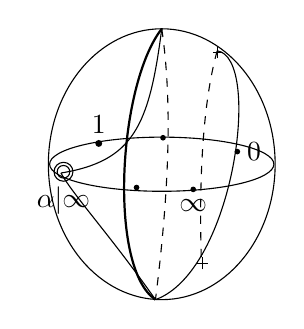
\begin{tikzpicture}[x=.8cm,y=.8cm]
\draw (0,0) ellipse (1.8 and 2.15);
\draw (0,0) ellipse (1.78 and .43);
\draw[thick] (0,2.15)..controls(-.7,1.25)and(-.85,-1.65)..(-.1,-2.15);
\draw[dashed] (0,2.15)..controls(.2,.8)and(.07,-.8)..(-.1,-2.15);
\draw (-.1,-2.15)..controls(1.15,-1.7)and(1.6,1.7)..(.88,1.8);
\draw[dashed] (.88,1.8)..controls(.6,.8)and(.6,-.7)..(.63,-1.55);
\draw (-1.6,-.14)..controls(-1.4,-.5)and(-.8,-1.15)..(-.1,-2.15);
\draw[thin] (-1.6,-.14)..controls(-.45,.05)and(-.2,.6)..(0,2.15);
\fill (-1,.33) circle (.055) node[above] {$1$};
\fill (1.2,.2) circle (.045) node[right] {$0$};
\fill (.5,-.4) circle (.045) node[below] {$\infty$};
\draw (-1.56,-.12) circle (.10); \draw (-1.56,-.12) circle (.15);
\node[below] at (-1.56,-.2) {$\unsure{\alpha|\infty}$};
\fill (-.4,-.37) circle (.045); \fill (.02,.42) circle (.045);
\draw (.81,1.77)--(.98,1.77) (.89,1.68)--(.89,1.87);
\draw (.55,-1.57)--(.73,-1.57) (.64,-1.67)--(.64,-1.48);
\end{tikzpicture}}

\[
\mathcal T_{0,4}^{+!}\simeq\Pi_{0,3}\quad\deleted{\unsure{m}}
\]
\diagram{\begin{tikzcd}[column sep=large,row sep=large]
1\arrow[r]&\Pi_{0,3}\arrow[r]\arrow[d,equal]&\mathcal T_{0,4}^{+}\arrow[r]\arrow[d,"{\mathrm{can}^{\unsure{t}}}"]&\widetilde{\mathfrak S}_4\arrow[r]\arrow[d,"\mathrm{can}"]&1\\
1\arrow[r]&\Pi_{0,3}\arrow[r,dash]&\mathcal T_{\unsure{0|1},1[\unsure{1}]}^{+}\arrow[r]\arrow[d,equal]&\widetilde{\mathfrak S}_3\arrow[r]\arrow[d,equal]&1\\
&&\mathrm{SL}(2,\mathbb Z)/\!\pm1&\mathrm{SL}(2,\mathbb Z/2\mathbb Z)&
\end{tikzcd}}
\[
\mathcal T_{0,4}^{+!}\simeq\mathcal T_{\unsure{0|1},1}^{+}/\!\pm1
\quad\begin{matrix}\Vert\\ \mathrm{SL}(2,\mathbb Z)/\!\pm1\end{matrix}
\]

\diagram{\begin{tikzcd}[column sep=large,row sep=large]
0\arrow[r]&\Pi_{0,3}\arrow[r]&\mathcal T_{\unsure{0|1},1}^{+}\arrow[r]\arrow[d,equal]&\deleted{\unsure{\mathbb Z\times\mathbb Z}}\ \widetilde{\mathfrak S}_3\arrow[r,dash]\arrow[d,equal]&1\\
&\deleted{\unsure{\ell_1\ \ell_0\ \ell_1\ \ell_2}}&\mathrm{SL}(2,\mathbb Z)&\mathrm{SL}(2,\mathbb Z/4\mathbb Z)/---&
\end{tikzcd}}
\[
\unsure{\mathrm{GL}|\mathrm{PGL}}(2,\mathbf F_2)
\]

\[
\mathrm{SL}(2,\mathbb Z)/\underbrace{(\pm1.\mathbb Z)}_{\text{\uline{Borel}}}
\simeq\unsure{\mathbf P^1_{\mathbb Z}|\mathbf P^1(\mathbb Z)}
\simeq\mathbf P^1(\mathbb Q)
\]
\diagram{\begin{tikzcd}
\unsure{\mathbf P^1_{\mathbb Z}|\mathbf P^1(\mathbb Z)}\arrow[d]\\
\mathbf P^1(\mathbb Z/2\mathbb Z)
\end{tikzcd}}
\[
\ell_0\ \ell_1\ \ell_2\ \ell_3=1
\]
\[
\ell_0\ell_1\ell_\infty=1\qquad
\ell_\infty=\ell'_\infty
\]
\[
\ell'_{\unsure{\infty|0}}\ell'_2\ell'_3=1
\]

\figure{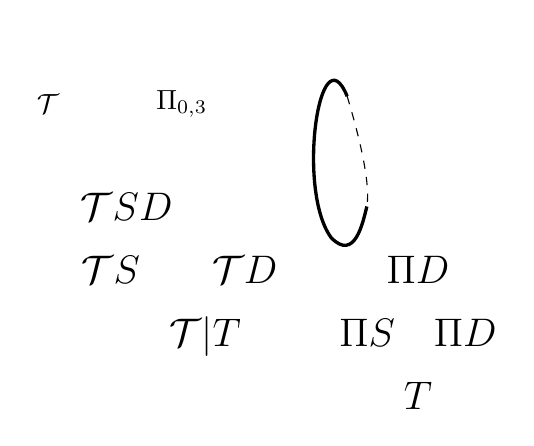
\begin{tikzpicture}[x=1cm,y=1cm]
\node at (0,1.4) {$\mathcal T$};
\node at (1.7,1.4) {$\Pi_{0,3}$};
\draw[very thick] (3.8,1.5)..controls(3.45,2.35)and(3.15,.3)..(3.6,-.3)..controls(3.9,-.6)and(4.0,-.1)..(4.05,.1);
\draw[dashed] (3.8,1.5)..controls(3.95,1.0)and(4.1,.4)..(4.05,.1);
\node[font=\Large] at (1.0,.1) {$\mathcal T S D$};
\node[font=\Large] at (.8,-.7) {$\mathcal T S$};
\node[font=\Large] at (2.5,-.7) {$\mathcal T D$};
\node[font=\Large] at (2.0,-1.55) {$\unsure{\mathcal T|\mathfrak T}$};
\node[font=\Large] at (4.7,-.7) {$\Pi D$};
\node[font=\Large] at (4.7,-1.5) {$\Pi S\quad\Pi D$};
\node[font=\Large] at (4.7,-2.3) {$\mathbb T$};
\end{tikzpicture}}

\[
\mathcal T_{0,4}^{+!}\qquad
\mathcal T^+\ \deleted{\unsure{\mathcal T}}
\]
\diagram{\begin{array}{ll}
\text{groupoïdes}&\mathcal T\\
\text{groupes}&T\\
\text{multiplicités}&M\\
\text{\uline{espaces} de T}&\widetilde M
\end{array}}
\[
T^+,\ T^!,\ T^{+!},\quad T/T^+
\qquad\mathrm{GL}(2,\mathbb Z)/\mathbb Z^*
\]

\diagram{\begin{tikzcd}[column sep=large,row sep=large]
1\arrow[r]&\Pi_{g,\nu-1}\arrow[r]&\unsure{\mathbb T|\mathcal T}_{g,\nu}\arrow[r]\arrow[d,"\simeq",phantom,sloped]&\underbrace{\unsure{\mathbb T|\mathcal T}_{g,\nu-1}}_{X_{g,\nu-1}}\arrow[r]&1\\
&&\Pi(\mathcal X_{g,\nu-1},\unsure{\mathbb T|\mathcal T}_{g,\nu-1};s_\nu)&&
\end{tikzcd}}
\[
X_{g,\nu-1}\subset\mathcal X
\]

\figure{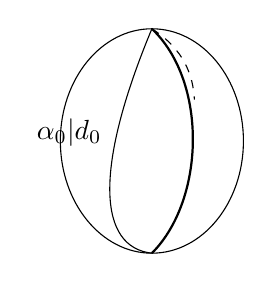
\begin{tikzpicture}[x=.75cm,y=.75cm]
\draw (0,0) ellipse (1.55 and 1.9);
\draw (0,1.9)..controls(-1,-.5)and(-.9,-1.8)..(0,-1.9);
\draw[thick] (0,1.9)..controls(.95,1)and(.9,-1)..(0,-1.9);
\draw[dashed] (0,1.9)..controls(.55,1.55)and(.7,1.1)..(.72,.7);
\node at (-1.4,.15) {$\unsure{\alpha_0|d_0}$};
\end{tikzpicture}}

\[
\unsure{\mathcal M|M}_{g,\nu}-
\]
\figure{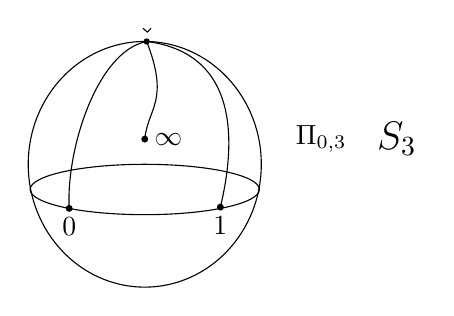
\begin{tikzpicture}[x=.8cm,y=.8cm]
\draw (0,0) ellipse (1.85 and 1.95);
\draw (0,-.4) ellipse (1.82 and .4);
\draw[thin] (.03,1.95)..controls(-.75,1.8)and(-1.25,.25)..(-1.2,-.7);
\draw (.03,1.95)..controls(1.6,1.75)and(1.4,.15)..(1.2,-.68);
\draw (.03,1.95)..controls(.4,1.0)and(.05,.9)..(0,.4);
\fill (.03,1.95) circle (.05); \draw(-.03,2.16)--(.04,2.1)--(.1,2.16);
\fill (-1.2,-.7) circle (.055) node[below] {$0$};
\fill (1.2,-.68) circle (.055) node[below] {$1$};
\fill (0,.4) circle (.055) node[right] {$\infty$};
\node at (2.8,.4) {$\Pi_{0,3}$}; \node[font=\Large] at (4.0,.4) {$\mathfrak S_3$};
\end{tikzpicture}}
